\documentclass[12pt]{../style-files/ociamthesis}

\usepackage{amssymb}
\usepackage{titlesec}
\usepackage{amsmath}
\usepackage{float}
\usepackage{graphicx}
\usepackage{caption}
\usepackage{subfig}
\usepackage{xcolor}
\usepackage[section]{placeins}
\usepackage{mathrsfs}
\usepackage{bm}
\usepackage{stmaryrd}
\usepackage{siunitx}
\usepackage{rotating}
\usepackage[utf8]{inputenc}
\usepackage[round]{natbib}
\usepackage{tikz}
\usetikzlibrary{fadings}
\usetikzlibrary{snakes}
\usepackage{booktabs}
\usepackage{multirow}

%%%%%%%%%%%%%%%%%%%%%%%%%%%%%%%%%%%%%%%%%%%%%%%%%%%%%%%%%%
% the following is to alter tikz settings to improve springs figure.
\usetikzlibrary{decorations.pathmorphing,calc,patterns}
\makeatletter
\def\pgfdecorationspringstraightlinelength{0.5cm}
\def\pgfdecorationspringnumberofelement{8}
\def\pgfdecorationspringnaturallength{5cm}
\pgfkeys{%
	/pgf/decoration/.cd,
	spring straight line length/.code={%
		\pgfmathsetlengthmacro\pgfdecorationspringstraightlinelength{#1}},
	spring natural length/.code={%
		\pgfmathsetlengthmacro\pgfdecorationspringnaturallength{#1}},
	spring number of element/.store in=\pgfdecorationspringnumberofelement
}

\pgfdeclaredecoration{coil spring}{straight line}{%
	\state{straight line}[%
	persistent precomputation = {%
		% Compute the effective length of the spring (without the length
		% of the two straight lines): \pgfdecorationspringeffectivelength
		\pgfmathsetlengthmacro{\pgfdecorationspringeffectivelength}%
		{\pgfdecoratedpathlength-2*\pgfdecorationspringstraightlinelength}
		% Compute the effective length of one coil pattern:
		% \pgfdecorationspringeffectivelengthofonecoil
		\pgfmathsetlengthmacro{\pgfdecorationspringeffectivelengthofonecoil}%
		{\pgfdecorationspringeffectivelength/\pgfdecorationspringnumberofelement}
	},
	width = \pgfdecorationspringstraightlinelength,
	next state = draw spring]{%
		\pgfpathlineto{%
			\pgfqpoint{%
				\pgfdecorationspringstraightlinelength}{0pt}}
	}
	\state{draw spring}%
	[width=\pgfdecorationspringeffectivelengthofonecoil,
	repeat state=\pgfdecorationspringnumberofelement-1,next state=final]{%
		\pgfpathcurveto
		{\pgfpoint@onspringcoil{0    }{ 0.555}{1}}
		{\pgfpoint@onspringcoil{0.445}{ 1    }{2}}
		{\pgfpoint@onspringcoil{1    }{ 1    }{3}}
		\pgfpathcurveto
		{\pgfpoint@onspringcoil{1.555}{ 1    }{4}}
		{\pgfpoint@onspringcoil{2    }{ 0.555}{5}}
		{\pgfpoint@onspringcoil{2    }{ 0    }{6}}
		\pgfpathcurveto
		{\pgfpoint@onspringcoil{2    }{-0.555}{7}}
		{\pgfpoint@onspringcoil{1.555}{-1    }{8}}
		{\pgfpoint@onspringcoil{1    }{-1    }{9}}
		\pgfpathcurveto
		{\pgfpoint@onspringcoil{0.445}{-1    }{10}}
		{\pgfpoint@onspringcoil{0    }{-0.555}{11}}
		{\pgfpoint@onspringcoil{0    }{ 0    }{12}}
	}
	\state{final}{%
		\pgfpathlineto{\pgfpointdecoratedpathlast}
	}
}

\def\pgfpoint@onspringcoil#1#2#3{%
	\pgf@x=#1\pgfdecorationsegmentamplitude%
	\pgf@x=.5\pgf@x%
	\pgf@y=#2\pgfdecorationsegmentamplitude%
	\pgfmathparse{0.083333333333*\pgfdecorationspringeffectivelengthofonecoil}%
	\pgf@xa=\pgfmathresult pt
	\advance\pgf@x by#3\pgf@xa%
}

\makeatother

\tikzset{%
	Spring/.style = {%
		decoration = {%
			coil spring,
			spring straight line length = 0.2cm,
			% To be added
			spring natural length = #1,
			spring number of element = 4,
			amplitude=2mm},
		decorate,
		very thick},
	Spring/.default = {4cm}}
%%%%%%%%%%%%%%%%%%%%%%%%%%%%%%%%%%%%%%%%%%%%%%%%%


\usepackage{geometry}
 \geometry{
 a4paper,
 left=40mm,
 right=30mm,
 top=30mm,
 bottom=30mm
 }

\definecolor{theblue}{HTML}{0000CD}

% disable this package for printed version
\usepackage[colorlinks=true, linktocpage=true, allcolors=theblue]{hyperref}

\titleformat{\chapter}[display]
  {\bfseries\Large}
  {\filright\MakeUppercase{\chaptertitlename} \Large\thechapter}
  {1ex}
  {}
  [\vspace{1ex} \hrule \vspace{1pt} \hrule]

\newcommand{\adv}{    {\it Adv. Space Res.}} 
\newcommand{\annG}{   {\it Ann. Geophys.}} 
\newcommand{\aap}{    {\it Astron. Astrophys.}}
\newcommand{\aaps}{   {\it Astron. Astrophys. Suppl.}}
\newcommand{\aapr}{   {\it Astron. Astrophys. Rev.}}
\newcommand{\ag}{     {\it Ann. Geophys.}}
\newcommand{\aj}{     {\it Astron. J.}} 
\newcommand{\apj}{    {\it Astrophys. J.}}
\newcommand{\apjl}{   {\it Astrophys. J. Lett.}}
\newcommand{\apss}{   {\it Astrophys. Space Sci.}} 
\newcommand{\cjaa}{   {\it Chin. J. Astron. Astrophys.}} 
\newcommand{\gafd}{   {\it Geophys. Astrophys. Fluid Dyn.}}
\newcommand{\grl}{    {\it Geophys. Res. Lett.}}
\newcommand{\ijga}{   {\it Int. J. Geomagn. Aeron.}}
\newcommand{\jastp}{  {\it J. Atmos. Solar-Terr. Phys.}} 
\newcommand{\jgr}{    {\it J. Geophys. Res.}}
\newcommand{\mnras}{  {\it Mon. Not. Roy. Astron. Soc.}}
\newcommand{\na}{     {\it New Astronomy}}
\newcommand{\nat}{    {\it Nature}}
\newcommand{\pasp}{   {\it Pub. Astron. Soc. Pac.}}
\newcommand{\pasj}{   {\it Pub. Astron. Soc. Japan}}
\newcommand{\pre}{    {\it Phys. Rev. E}}
\newcommand{\solphys}{{\it Solar Phys.}}
\newcommand{\sovast}{ {\it Soviet  Astron.}} 
\newcommand{\ssr}{    {\it Space Sci. Rev.}}
\newcommand{\caa}{    {\it Chinese Astron. Astrohpys.}} 
\newcommand{\apjs}{   {\it Astrophys. J. Suppl.}}

\begin{document}

\baselineskip=18pt

\setcounter{secnumdepth}{3}
\setcounter{tocdepth}{3}

\setcounter{chapter}{1}


\newcommand{\bv}{\mathbf{v}}
\newcommand{\bB}{\mathbf{B}}


\newcommand{\figdir}{../main/figures/chpt-2/} % where figures are stored

%------------------------------------------------------------------------------
\chapter{Asymmetric waveguides - eigenvalue problem}
\label{chap: EVP}
%------------------------------------------------------------------------------


%------------------------------------------------------------------------------
\section{Chapter introduction}
\label{sec: EVP intro}
%------------------------------------------------------------------------------

The simplest model of an asymmetric waveguide is an asymmetric magnetic slab in a non-magnetic environment\footnote{More precisely, the simplest model of an asymmetric MHD waveguide is an interface between different plasmas; the asymmetric slab is the simplest asymmetric waveguide that can oscillate in a collective body mode (see Section~\ref{sec: body}).}

Section~\ref{sec: EVP non-mag} is based on \cite{all_etal17} and Section~\ref{sec: EVP mag} is based on \cite{zsa_etal18}.

%------------------------------------------------------------------------------
\section{Asymmetric slab}
\label{sec: asym slab}
%------------------------------------------------------------------------------
\subsection{Model description}
Figure~\ref{fig: eq} illustrates the construction of this mathematical model, where a three-dimensional, unbounded, inviscid plasma is separated into three regions by two parallel planar interfaces at $x = \pm x_0$. The equilibrium magnetic field is in the $z$-direction and has magnitude
\begin{equation}
	B(x)=
	\begin{cases}
		B_1 & \text{if } x < -x_0, \\
		B_0 & \text{if } |x|\leq{x_0}, \\
		B_2 & \text{if } x > x_0,
	\end{cases}
\end{equation}
where $B_j$, for $j = 0, 1, 2$ are constant. Within each region, denoted by subscripts 0, 1, and 2, the plasma is uniform and the equilibrium plasma pressure, density, and temperature are denoted by $p_j$, $\rho_j$, and $T_j$, respectively, for $j = 0, 1, 2$. This defines an \textit{isolated} waveguide, by which we mean there is no adjacent waveguides that can effect the oscillations.

\begin{figure}
	\centering
	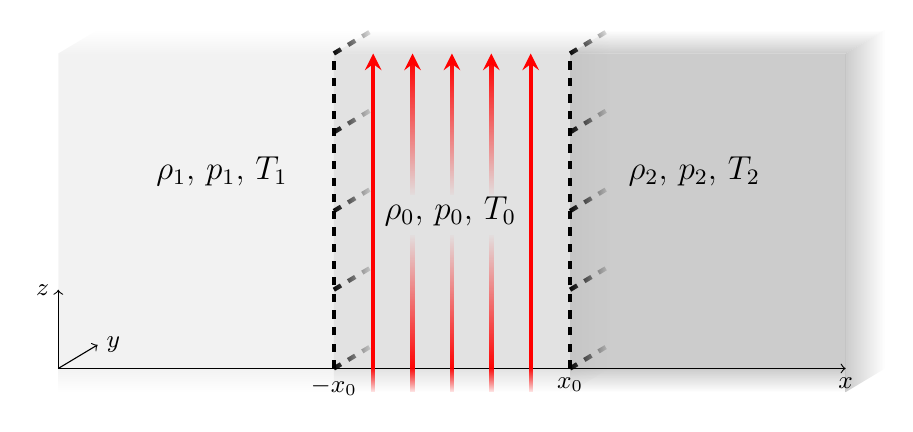
\begin{tikzpicture}
	\path [fill=lightgray, opacity=0.45] (3.5,0) -- (3.5,4) -- (6.5,4) -- (6.5,0) -- (3.5,0);
	\shade[left color=lightgray,right color=white, opacity=0.45] (6.5,0) -- (6.5,4) -- (7,4.3) -- (7,0.3) -- (6.5,0);
	\shade[top color=lightgray,bottom color=white, opacity=0.45] (3.5,0) -- (6.5,0) -- (6.5,-0.3) -- (3.5,-0.3) -- (3.5,0);
	\shade[top color=white,bottom color=lightgray, opacity=0.45] (3.5,4) -- (4,4.3) -- (7,4.3) -- (6.5,4) -- (3.5,4);
	\shade[left color=lightgray,right color=white, opacity=0.45] (6.5,0) -- (6.5,-0.3) -- (7,0) -- (7,0.3) -- (6.5,0);
	
	\path [fill=lightgray, opacity=0.8] (6.5,0) -- (6.5,4) -- (10,4) -- (10,0) -- (6.5,0);
	\shade[top color=lightgray,bottom color=white, opacity=0.8] (6.5,0) -- (10,0) -- (10,-0.3) -- (6.5,-0.3) -- (6.5,0);
	\shade[top color=white,bottom color=lightgray, opacity=0.8] (6.5,4) -- (7,4.3) -- (10.5,4.3) -- (10,4) -- (6.5,4);
	\shade[left color=lightgray,right color=white, opacity=0.8] (10,-0.3) -- (10,4) -- (10.5,4.3) -- (10.5,0) -- (10,-0.3);
	
	\path [fill=lightgray, opacity=0.2] (0,0) -- (0,4) -- (3.5,4) -- (3.5,0) -- (0,0);
	\shade[top color=lightgray,bottom color=white, opacity=0.2] (0,0) -- (3.5,0) -- (3.5,-0.3) -- (0,-0.3) -- (0,0);
	\shade[top color=white,bottom color=lightgray, opacity=0.2] (0,4) -- (0.5,4.3) -- (4,4.3) -- (3.5,4) -- (0,4);
	
	\draw [<->] (0,1) -- (0,0) -- (10,0);
	\draw [->] (0,0) -- (0.5,0.3);
	
	\draw [ultra thick, dashed] (3.5,0) -- (3.5,4);
	\draw [ultra thick, dashed, path fading=east] (3.5,0) -- (4,0.3);
	\draw [ultra thick, dashed, path fading=east] (3.5,4) -- (4,4.3);
	\draw [ultra thick, dashed, path fading=east] (3.5,2) -- (4,2.3);
	\draw [ultra thick, dashed, path fading=east] (3.5,1) -- (4,1.3);
	\draw [ultra thick, dashed, path fading=east] (3.5,3) -- (4,3.3);
	\draw [ultra thick, red, -stealth] (4,0) -- (4,4);
	\draw [ultra thick, red, path fading=south] (4,-0.3) -- (4,0);
	\draw [ultra thick, red, path fading=north] (4.5,0) -- (4.5, 1.7);
	\draw [ultra thick, red, path fading=south] (4.5,-0.3) -- (4.5,0);
	\draw [ultra thick, red, path fading=south] (4.5,2.2) -- (4.5,3.9);
	\draw [ultra thick, red, -stealth] (4.5,3.9) -- (4.5,4);
	\draw [ultra thick, red, path fading=north] (5,0) -- (5, 1.7);
	\draw [ultra thick, red, path fading=south] (5,-0.3) -- (5, 0);
	\draw [ultra thick, red, path fading=south] (5,2.2) -- (5,3.9);
	\draw [ultra thick, red, -stealth] (5,3.9) -- (5,4);
	\draw [ultra thick, red, path fading=north] (5.5,0) -- (5.5, 1.7);
	\draw [ultra thick, red, path fading=south] (5.5,-0.3) -- (5.5, 0);
	\draw [ultra thick, red, path fading=south] (5.5,2.2) -- (5.5,3.9);
	\draw [ultra thick, red, -stealth] (5.5,3.9) -- (5.5,4);
	\draw [ultra thick, red, -stealth] (6,0) -- (6,4);
	\draw [ultra thick, red, path fading=south] (6,-0.3) -- (6,0);
	\draw [ultra thick, dashed] (6.5,0) --(6.5,4);
	\draw [ultra thick, dashed, path fading=east] (6.5,0) -- (7,0.3);
	\draw [ultra thick, dashed, path fading=east] (6.5,4) -- (7,4.3);
	\draw [ultra thick, dashed, path fading=east] (6.5,2) -- (7,2.3);
	\draw [ultra thick, dashed, path fading=east] (6.5,1) -- (7,1.3);
	\draw [ultra thick, dashed, path fading=east] (6.5,3) -- (7,3.3);
	
	\small
	\node [below] at (3.5,0) {$-x_0$};
	\node [below] at (6.5,0) {$x_0$};
	\node [below] at (10,0) {$x$};
	\node [left] at (0,1) {$z$};
	\node [right] at (0.5,0.3) {$y$};
	
	\large
	\node [right] at (1.1,2.5) {$\rho_1$, $p_1$, $T_1$};
	\node [right] at (4,2) {$\rho_0$, $p_0$, $T_0$};
	\node [right] at (7.1,2.5) {$\rho_2$, $p_2$, $T_2$};
	\end{tikzpicture}
	\caption{The equilibrium state inside the slab, ($|x| \leq x_0$) and outside the slab, ($x < -x_0$ and $x > x_0$). The red arrows illustrate magnetic field lines, $B(x)\mathbf{\widehat{z}}$, and the dashed black lines indicate the boundaries of the slab. \textcolor{red}{Change to mag outside}}
	\label{fig: eq}
\end{figure}

To ensure that the model is in equilibrium, the total pressure in each external region must balance the total pressure in the internal region, namely
\begin{equation}
	p_1 + \frac{B_1^2}{2\mu_0} = p_0 + \frac{B_0^2}{2\mu_0} = p_2 + \frac{B_2^2}{2\mu_0}, \label{pressure balance}
\end{equation}
where $\mu_0$ is the permeability of free space. We can rewrite Equation~\eqref{pressure balance} as
\begin{equation}
\rho_i\left(c_i^2 + \frac{\gamma}{2}v_{Ai}^2\right) = \rho_j\left(c_j^2 + \frac{\gamma}{2}v_{Aj}^2\right), \quad \text{for} \quad i, j = 0, 1, 2, \label{sound speeds}
\end{equation}
where we define the sound and Alfv\'{e}n speeds in each region by $c_j = \sqrt{\gamma p_j/\rho_j}$ and $v_{Aj} = B_j/\sqrt{\mu\rho_j}$, respectively, for $j = 0, 1, 2$. The adiabatic index\footnote{The adiabatic index is assumed uniform across the whole domain under the single-fluid approximation.} is $\gamma$.


\subsection{The dispersion relation}

In the derivation of the dispersion relation, we decompose the linearised ideal MHD equations into Fourier forms then combine them into an ordinary differential equation (ODE) for the transverse velocity perturbation for each of the three plasma regions. After finding the general solution to each of these ODEs, we match the solutions across each interface at $\pm x_0$. The condition for the existence of non-trivial solutions will lead to the dispersion relation. In mathematical terms, we're converting a set of partial differential equations into ordinary differential equations into algebraic equations, into a single equation. From a form that we cannot solve into a form that we can.


\subsubsection{Derivation} \label{sec: asym slab DR der}

We begin with the ideal MHD equations, linearised around a static equilibrium with subscripts $j$, Equations~\eqref{cont eqn lin}-\eqref{ind eqn lin}. Taking the partial derivative with respect to time of Equation~\eqref{mom eqn lin} and eliminating $\bB$ using Equation~\eqref{ind eqn lin}, gives \textcolor{red}{Check whether the last - should be a + in the first two eqns below.}
\begin{align}
	\frac{\partial^2 v_x}{\partial t^2} &= \frac{\partial}{\partial x}\left[ (c_j^2 + v_{Aj}^2)\nabla\cdot\bv - v_{Aj}^2\frac{\partial v_z}{\partial z} \right] + v_{Aj}^2 \frac{\partial^2 v_x}{\partial z^2} \label{mom x} \\
	\frac{\partial^2 v_y}{\partial t^2} &= \frac{\partial}{\partial y}\left[ (c_j^2 + v_{Aj}^2)\nabla\cdot\bv - v_{Aj}^2\frac{\partial v_z}{\partial z} \right] + v_{Aj}^2 \frac{\partial^2 v_y}{\partial z^2} \label{mom y} \\
	\frac{\partial^2 v_z}{\partial t^2} &= c_j^2\frac{\partial}{\partial z}(\nabla\cdot\bv). \label{mom z}
\end{align}
Taking Fourier solutions like $f(\mathbf{x},t) = \hat{f}(x) \exp{i(ly + kz - \omega t)}$, where $\mathbf{k} = (0, l, k)$ is the wavenumber vector and $\omega$ is the angular frequency, for $\mathbf{v}$ in Equation~\eqref{mom y} gives
\begin{equation}
(k^2v_{Aj}^2 - \omega^2)\hat{v}_y = l((c_j^2 + v_{Aj}^2)(i\hat{v}_x' - l\hat{v}_y - k\hat{v}_z) + kv_{Aj}^2\hat{v}_z),
\end{equation}
where $' = d/dx$. If the component of the wavenumber in the $y$-direction is zero, \textit{i.e.} $l = 0$, then this equation reduces to
\begin{equation}
(k^2v_{Aj}^2 - \omega^2)\hat{v}_y(x) = 0,
\end{equation}
which yield two solutions. Firstly, $\omega^2 = k^2v_{Aj}^2$ is a solution corresponding to shear Alfv\'{e}n waves with different phase speed for each magnetic iso-surface (in this case surfaces parallel to the $yz$-plane). The second solution is $\hat{v}_y(x) = 0$ for all $x$ and therefore $v_y = 0$, \textit{i.e.} waves without perturbation component along the slab and perpendicular to the magnetic field. These solutions correspond to magneto-acoustic modes. Thus we have a decoupling of the shear Alfv\'{e}n modes from the magneto-acoustic modes.

Focusing from here on magneto-acoustic modes, we seek solutions of the Fourier form
\begin{equation}
\bv(\mathbf{x},t)=(\hat{v}_x(x)\textrm{e}^{i(kz-\omega{t})}, 0, \hat{v}_z(x)\textrm{e}^{i(kz-\omega{t})}),
\label{vcomponents}
\end{equation}
This restricts the investigation to magneto-acoustic waves propagating parallel to the equilibrium magnetic field, with velocity perturbation amplitude $\hat{v}_x(x)$ in the $x$-direction, and $\hat{v}_z(x)$ in the $z$-direction. With this ansatz, Equation~\eqref{mom y} degenerates and Equations~\eqref{mom x} and~\eqref{mom z} become
\begin{align}
&-\omega^2\hat{v}_x = (c_j^2+v_\textrm{Aj}^2)(\hat{v}_x'' + ik\hat{v}_z') - v_\textrm{Aj}^2ik\hat{v}_z'-v_\textrm{Aj}^2k^2\hat{v}_x, \label{mom x 2} \\
&-\omega^2\hat{v}_z = c_j^2ik(\hat{v}_x' + ik\hat{v}_z). \label{mom z 2}
\end{align}
These equations can be combined to give an ordinary differential equation for $\hat{v}_x$, namely
\begin{equation}
\hat{v}_x'' - m_j^2\hat{v}_x = 0, \quad \text{where} \quad
m_j^2 = \frac{(k^2v_\textrm{Aj}^2 - \omega^2)(k^2c_j^2 - \omega^2)}{(c_j^2 + v_\textrm{Aj}^2)(k^2c_\textrm{Tj}^2 - \omega^2)}. \label{v_x ODE}
\end{equation}
This is identical to the corresponding equation governing, for example, a tangential interface or a symmetric slab, derived in Sections~\ref{sec: MHD waves interface} and~\ref{sec: MHD waves sym slab} by \cite{rob81a,edw_etal82}.

Solutions of Equations~\eqref{v_x ODE} are a linear combination of hyperbolic functions. We restrict our model to waves trapped by the slab by imposing the boundary condition $\hat{v}_x \to 0$ as $|x| \to \infty$. Thus, the general solution for the velocity perturbation in the $x$-direction is
\begin{equation}
\hat{v}_x(x)=
\begin{cases}
A(\cosh{m_1x} + \sinh{m_1x}), & \text{if } x < -x_0, \\
B\cosh{m_0x} + C\sinh{m_0x}, & \text{if } |x| \leq {x_0}, \\
D(\cosh{m_2x} - \sinh{m_2x}), & \text{if  } x > x_0, 
\end{cases} \label{vsoln}
\end{equation}
where $A$, $B$, $C$, and $D$ are arbitrary constants (with respect to $x$). The remaining boundary conditions are continuity of velocity and total pressure across the slab boundaries at $x = \pm{x_0}$. With the aim of finding an expression for the total pressure perturbation, the Equations~\eqref{cont eqn lin} and~\eqref{energy eqn lin} can be combined to give
\begin{equation}
	\frac{\partial p}{\partial t} = - \rho_jc_i^2\nabla\cdot\bv.
\end{equation}
Using the above equation and the $z$-component of Equation~\eqref{ind eqn lin}, the perturbation in total pressure (plasma pressure, $p$, plus magnetic pressure, $B_jB_z/\mu$) across the whole domain can be shown to have amplitude
\begin{equation}
\hat{p}_T(x) = \frac{\Lambda_j}{m_j}\hat{v}_x'(x),
\end{equation}
where
\begin{equation}
\Lambda_j = \frac{i\rho_j(\omega^2 - \omega_{Aj}^2)}{m_j\omega}, \quad \text{for} \quad j = 0, 1, 2. \label{Lambdas}
\end{equation}
Ensuring continuity of velocity and total pressure across the slab boundaries gives four coupled algebraic equations, namely
\begin{equation}
\left(
\begin{matrix}
c_1-s_1             &-c_0           &s_0            &0                   \\
0                   &c_0            &s_0            &s_2-c_2             \\
\Lambda_1(c_1-s_1)  &\Lambda_0s_0   &-\Lambda_0c_0  &0                   \\
0                   &\Lambda_0s_0   &\Lambda_0c_0   &-\Lambda_2(s_2-c_2)
\end{matrix}
\right)
\left(
\begin{matrix}
A \\
B \\
C \\
D
\end{matrix}
\right)
=
\left(
\begin{matrix}
0 \\
0 \\
0 \\
0
\end{matrix}
\right),
\label{coefmatrix}
\end{equation}
where $c_j = \cosh{m_jx_0}$ and $s_j = \sinh{m_jx_0}$ for $j=0,1,2$, for brevity. The condition for the existence of non-trivial solutions to this system of equations is that the determinant of the matrix is zero. Applying this condition gives us the dispersion relation for an asymmetric slab, namely
\begin{equation}
(\Lambda_0^2 + \Lambda_1\Lambda_2) + \Lambda_0(\Lambda_1 + \Lambda_2)\coth{2m_0x_0} = 0. \label{DR lambda}
\end{equation}
By expanding each $\Lambda_j$, we can write this dispersion relation in familiar variables as
\begin{align}
&m_0^2(\omega^2 - \omega_{A1}^2)(\omega^2 - \omega_{A2}^2) + \frac{\rho_0}{\rho_1}m_1\frac{\rho_0}{\rho_2}m_2(\omega^2 - \omega_{A0}^2)^2 \notag \\
& + m_0(\omega^2 - \omega_{A0}^2)\left[\frac{\rho_0}{\rho_1}m_1(\omega^2 - \omega_{A2}^2) + \frac{\rho_0}{\rho_2}m_2(\omega^2 - \omega_{A1}^2)\right]\coth{2m_0x_0} = 0. \label{DR}
\end{align}


\subsubsection{First-order asymmetric slab}

There is a qualitative difference between waves propagating along symmetric and asymmetric magnetic slabs. The dispersion relation governing an asymmetric slab is a single equation, whereas the dispersion relation governing a symmetric slab \citep{rob81a} consists of two independent equations, corresponding to the sausage and kink eigenmodes.

Under the approximation that the densities and temperatures of the external plasma are of the same order, the dispersion relation, Equation~\eqref{DR}, can be factorised to give the approximate dispersion relation
\begin{equation}
\left[\Lambda_0(\Lambda_1+\Lambda_2)+2\Lambda_1\Lambda_2\tanh{m_0x_0}\right]\left[\Lambda_0(\Lambda_1+\Lambda_2)+2\Lambda_1\Lambda_2\coth{m_0x_0}\right]=0. \label{DR approx lambda}
\end{equation}
To show this, define each bracket as the following functions
\begin{align}
D_s(\omega) &:= \Lambda_0(\Lambda_1 + \Lambda_2) + 2\Lambda_1\Lambda_2\tanh{m_0x_0}, \\
D_k(\omega) &:= \Lambda_0 (\Lambda_1 + \Lambda_2) + 2\Lambda_1\Lambda_2\coth{m_0x_0}.
\end{align}
There product is
\begin{align}
D_s(\omega)D_k(\omega) &= \left[ \Lambda_0(\Lambda_1 + \Lambda_2) + 2\Lambda_1\Lambda_2\tanh{m_0x_0} \right] \left[ \Lambda_0 (\Lambda_1 + \Lambda_2) + 2\Lambda_1\Lambda_2\coth{m_0x_0} \right] \\
&= \Lambda_0^2 (\Lambda_1 + \Lambda_2)^2 + 2\Lambda_0(\Lambda_1 + \Lambda_2)\Lambda_1\Lambda_2(\tanh{m_0x_0} + \coth{m_0x_0}) + 4\Lambda_1^2\Lambda_2^2 \\
&= 4\Lambda_1\Lambda_2 \left[ (\Lambda_0^2F + \Lambda_1\Lambda_2) + \Lambda_0(\Lambda_1 + \Lambda_2)\coth(2m_0x_0) \right] \\
\end{align}
where
\begin{equation}
F = \frac{(\Lambda_1 + \Lambda_2)^2}{4\Lambda_1\Lambda_2}.
\end{equation}
When the plasma parameters on each side of the slab are approximately equal, \textit{i.e.} $\Lambda_2 = \Lambda_1 (1 + \epsilon L)$, with $\epsilon \ll 1$ and $L \approx 1$, $F$ becomes
\begin{equation}
F = \frac{(2 + \epsilon L)^2}{4(1 + \epsilon L)} = 1 + \mathcal{O}(\epsilon^2).
\end{equation}
Therefore, 
\begin{equation}
(\Lambda_0^2 + \Lambda_1\Lambda_2) + \Lambda_0(\Lambda_1 + \Lambda_2)\coth(2m_0x_0) = \frac{1}{4\Lambda_1\Lambda_2} D_s(\omega) D_k(\omega) + \mathcal{O}(\epsilon^2).
\end{equation}
Therefore, to linear order of waveguide asymmetry, if the dispersion relation, Equation~\eqref{DR lambda} is satisfied, then either $D_s(\omega) = 0$ or $D_k(\omega) = 0$, which completes the proof of Equation~\eqref{DR approx lambda}.

The expressions for the variables $\Lambda_i$ for $i=0,1,2$ in Equations~\eqref{Lambdas} can be employed to yield the approximately symmetric dispersion relation
\begin{equation}
(\omega^2 - \omega_{A0}^2)\left(\frac{\rho_0}{\rho_1}\frac{m_1}{(\omega^2 - \omega_{A1}^2)} + \frac{\rho_0}{\rho_2}\frac{m_2}{(\omega^2 - \omega_{A2}^2)}\right) + 2m_0\left(\begin{matrix}\tanh \\ \coth \end{matrix}\right)(m_0x_0) = 0. \label{DR approx}
\end{equation}
This equation is now in a form similar to Equation~\eqref{DR sym slab}, the dispersion relation corresponding to MHD waves along a symmetric magnetic slab (Section~\ref{sec: MHD waves sym slab}), namely
\begin{equation}
\rho_im_e(\omega^2 - \omega_\textrm{Ai}^2) + \rho_em_i(\omega^2 - \omega_\textrm{Ae}^2)\left(\begin{matrix}\tanh \\ \coth \end{matrix}\right)(m_ix_0) = 0, \label{DRsym}
\end{equation}
where internal and external parameters are denoted by subscripts $i$ and $e$.


\subsection{Asymmetric eigenmodes}
There is a rich spectrum of MHD eigenmodes on an asymmetric magnetic slab. The key distinctions of these modes from the eigenmodes of a symmetric slab are discussed in this subsection. To aid the reader's understanding, we have created over a hundred 3D animations of symmetric and asymmetric eigenmodes in a magnetic slab \cite{all_etal18c}. The videos visualise the oscillations in the slab boundaries, magnetic field, density, and velocity field. \textcolor{red}{Consider including figure screenshots of the videos and describing/explaining them.}

The dispersion relation for a symmetric slab, Equation~\eqref{DRsym}, consists of two decoupled equations that correspond to the two types of eigenmodes supported by the slab: the \textit{sausage} and \textit{kink} MHD waves. In an asymmetric slab, the sausage and kink modes are modified by the external density difference, causing an asymmetry of the oscillation amplitude on each side of the slab (for visualisation see Figures~\ref{fig:saus} and~\ref{fig:kink}). We call these asymmetric eigenmodes quasi-sausage and quasi-kink modes. In a symmetric slab, sausage modes are characterised by an undisplaced slab axis in the centre of the slab. In an asymmetric slab, this undisplaced position is shifted towards the side of greatest external density for kink modes and towards the side of lowest external density for sausage modes. For symmetric kink modes, the width of the perturbed slab remains constant along the slab, but this characteristic is lost in an asymmetric slab. This highlights the mixed nature of these modes. 

Additionally, this shows that it is the phase of the boundary oscillations that is a more fundamental distinguishing characteristic of sausage and kink modes. For this reason, when we refer to \textit{sausage} and \textit{kink} modes of an asymmetric slab, we refer strictly to modes with boundary oscillations in \textit{anti-phase} and \textit{in-phase}, respectively. The differences between symmetric and asymmetric eigenmodes are summarised in Table~\ref{tab: eigenmode differences}.

\begin{figure}
	\makebox[\textwidth][c]{
		\subfloat[Quasi-kink]{\scalebox{1}{
				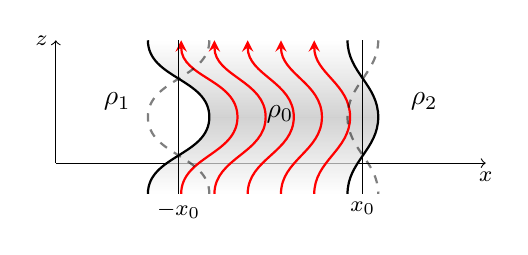
\begin{tikzpicture}[scale=0.78]
				\draw [->] (0,0) -- (7,0);
				
				\shade[bottom color=lightgray,top color=white, opacity=0.7] (1.5,2) to [out=-90,in=90] (2.5,0.75) to (5.25,0.75) to [out=90,in=-90] (4.75,2) to (1.5,2);
				
				\shade[bottom color=white,top color=lightgray, opacity=0.7] (2.5,0.75) to (5.25,0.75) to [out=-90,in=90] (4.75,-0.5) to (1.5,-0.5) to [out=90,in=-90] (2.5,0.75);
				
				\draw [thick] (1.5,2) to [out=-90,in=90] (2.5,0.75) to [out=-90,in=90] (1.5,-0.5);
				\draw [thick] (4.75,2) to [out=-90,in=90] (5.25,0.75) to [out=-90,in=90] (4.75,-0.5);
				
				\draw [thick, red, -stealth] (2.0417,-0.5) to [out=90,in=-90] (2.9583, 0.75) to [out=90,in=-90] (2.0417,2);
				\draw [thick, red, -stealth] (2.5833,-0.5) to [out=90,in=-90] (3.4167, 0.75) to [out=90,in=-90] (2.5833,2);
				\draw [thick, red, -stealth] (3.125,-0.5) to [out=90,in=-90] (3.875, 0.75) to [out=90,in=-90] (3.125,2);
				\draw [thick, red, -stealth] (3.6667,-0.5) to [out=90,in=-90] (4.3333, 0.75) to [out=90,in=-90] (3.6667,2);
				\draw [thick, red, -stealth] (4.2083,-0.5) to [out=90,in=-90] (4.7917, 0.75) to [out=90,in=-90] (4.2083,2);
				
				\draw [thick, dashed, opacity=0.5] (2.5,2) to [out=-90,in=90] (1.5,0.75) to [out=-90,in=90] (2.5,-0.5);
				\draw [thick, dashed, opacity=0.5] (5.25,2) to [out=-90,in=90] (4.75,0.75) to [out=-90,in=90] (5.25,-0.5);
				
				% % % % % % % % % % % % % % % % % % % % % % % % % %
				
				\draw [->] (0,0) -- (0,2);
				
				\node at (1,1) {$\rho_1$};
				\node at (6,1) {$\rho_2$};
				\node at (3.65,0.8) {$\rho_0$};
				
				\footnotesize
				\node [below] at (2,-0.5) {$-x_0$};
				\node [below] at (5,-0.5) {$x_0$};
				
				\node [left] at (0,2) {$z$};
				\node [below] at (7,0) {$x$};
				\draw [-] (2,-0.5) -- (2,2);
				\draw [-] (5,-0.5) -- (5,2);
				\end{tikzpicture}
				\label{fig:saus}}}
		%
		%
		%
		%
		\subfloat[Quasi-sausage]{\scalebox{1}{
				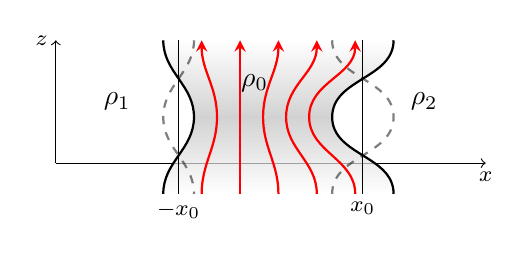
\begin{tikzpicture}[scale=0.78]
				\draw [->] (0,0) -- (7,0);
				
				\shade[bottom color=lightgray,top color=white, opacity=0.7] (1.75,2) to [out=-90,in=90] (2.25,0.75) to (4.5,0.75) to [out=90,in=-90] (5.5,2) to (1.75,2);
				
				\shade[bottom color=white,top color=lightgray, opacity=0.7] (2.25,0.75) to (4.5,0.75) to [out=-90,in=90] (5.5,-0.5) to (1.75,-0.5) to [out=90,in=-90] (2.25,0.75);
				
				\draw [thick] (1.75,2) to [out=-90,in=90] (2.25,0.75) to [out=-90,in=90] (1.75,-0.5);
				\draw [thick, dashed, opacity=0.5] (4.5,2) to [out=-90,in=90] (5.5,0.75) to [out=-90,in=90] (4.5,-0.5);
				
				\draw [thick, red, -stealth] (2.375,-0.5) to [out=90,in=-90] (2.625, 0.75) to [out=90,in=-90] (2.375,2);
				\draw [thick, red, -stealth] (3,-0.5) to [out=90,in=-90] (3, 0.75) to [out=90,in=-90] (3,2);
				\draw [thick, red, -stealth] (3.625,-0.5) to [out=90,in=-90] (3.375, 0.75) to [out=90,in=-90] (3.625,2);
				\draw [thick, red, -stealth] (4.25,-0.5) to [out=90,in=-90] (3.75, 0.75) to [out=90,in=-90] (4.25,2);
				\draw [thick, red, -stealth] (4.875,-0.5) to [out=90,in=-90] (4.125, 0.75) to [out=90,in=-90] (4.875,2);
				
				\draw [thick, dashed, opacity=0.5] (2.25,2) to [out=-90,in=90] (1.75,0.75) to [out=-90,in=90] (2.25,-0.5);
				\draw [thick] (5.5,2) to [out=-90,in=90] (4.5,0.75) to [out=-90,in=90] (5.5,-0.5);
				
				% % % % % % % % % % % % % % % % % % % % % % % % % %
				
				\draw [->] (0,0) -- (0,2);
				
				\node at (1,1) {$\rho_1$};
				\node at (6,1) {$\rho_2$};
				\node [right] at (2.86,1.3) {$\rho_0$};
				
				\footnotesize
				\node [below] at (2,-0.5) {$-x_0$};
				\node [below] at (5,-0.5) {$x_0$};
				
				\node [left] at (0,2) {$z$};
				\node [below] at (7,0) {$x$};
				\draw [-] (2,-0.5) -- (2,2);
				\draw [-] (5,-0.5) -- (5,2);
				\end{tikzpicture}
				\label{fig:kink}}}}
	\caption{Quasi-kink and quasi-sausage modes with external density ordering $\rho_1>\rho_2$. The red lines illustrate the perturbed magnetic field, the thick solid black lines illustrate the perturbed slab boundaries, and the dashed lines illustrate the future position of the slab boundaries after half a period. \textcolor{red}{remove arrows}}
\end{figure}

Sausage and kink modes are further categorised into \textit{surface} and \textit{body} modes. Surface modes are waves more enhanced at the slab boundaries, whereas body waves are characterised by oscillations permeating spatially throughout the slab, having their maximum amplitude within the slab. Mathematically, surface waves correspond to exponentially damped solutions of Equation~\eqref{vsoln} within the slab. This occurs when $m_0^2 > 0$, which occurs when the phase speed, $\omega/k$, satisfies
\begin{equation}
\frac{\omega}{k}<c_\textrm{T} \quad \text{or} \quad \text{min}\{c_0, v_\textrm{A}\}<\frac{\omega}{k}<\text{max}\{c_0, v_\textrm{A}\}.
\end{equation}
Body waves correspond to trigonometric solutions of Equation~\eqref{vsoln} within the slab. Most notably, this means that there are any number of nodes within the slab where the plasma is unperturbed, so that there exist an infinite set of body eigenmodes. They exist when $m_0^2 < 0$, which occurs when
\begin{equation}
c_\textrm{T}<\frac{\omega}{k}<\text{min}\{c_0, v_\textrm{A}\} \quad \text{or} \quad \text{max}\{c_0, v_\textrm{A}\}<\frac{\omega}{k}. \label{bconditions}
\end{equation}

For a surface mode (Figures~\ref{fig:surf quasi-kink} and~\ref{fig:surf quasi-saus}), the wave power distribution across the slab has a single minimum. The displacement of this minimum from the centre of the slab is a consequence of the asymmetry in the external plasma. The intensity of the maximum amplitudes on the left and right boundaries of the slab is different, reflecting the asymmetry in the external plasma.

Body modes are also affected by the asymmetric external environment (Figures~\ref{fig:body quasi-kink} and~\ref{fig:body quasi-saus}). Local maxima and minima in wave power are shifted towards the external plasma of higher density for a quasi-kink body mode and towards the external plasma of lower density for a quasi-sausage mode. However, this is a much weaker effect than for surface modes because the eigenfrequencies of body waves do not depend strongly on the parameters of the external plasma, and therefore they do not depend strongly on the asymmetry of the waveguide, as shown in Sections~\ref{sec: analytical solutions} and~\ref{sec: numerical solutions}. The same can be said for the eigenfunctions of body modes. These results corroborate the intuition that because the majority of the wave power is confined to within the slab, rather than its boundaries, the body modes don't \textit{feel} the external plasma as much as surface waves do.

\begin{table}
	\centering
	\begin{tabular}{ccccc}
		\toprule
		\multirow{2}{*}{Mode type} & Boundary & Constant & Axis & Unperturbed \\
		 & oscillations & width & displacement & position \\
		\midrule
		Symmetric sausage & Anti-phase & No & No & Middle \\
		Asymmetric sausage & Anti-phase & No & Yes & Shifted \\
		Symmetric kink & In-phase & Yes & Yes & - \\
		Asymmetric kink & In-phase & No	& Yes & - \\
		\bottomrule
	\end{tabular}
	\caption{The qualitative differences between symmetric and asymmetric surface modes.}
	\label{tab: eigenmode differences}
\end{table}

\begin{figure}
	\makebox[\textwidth][c]{
		\subfloat[Quasi-kink surface mode]{\scalebox{1}{
				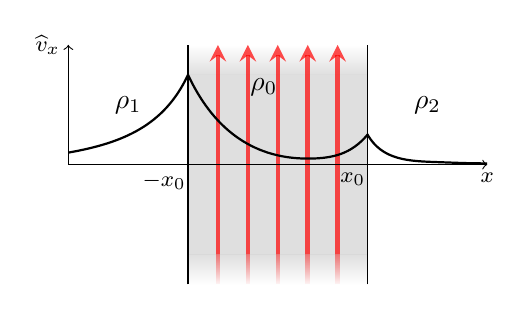
\begin{tikzpicture}[scale=0.76]
				\path [fill=lightgray, opacity=0.5] (2,-1.5) -- (2,1.5) -- (5,1.5) -- (5,-1.5) -- (2,-1.5);
				
				\shade[bottom color=white,top color=lightgray, opacity=0.5] (2,-2) to (5,-2) to (5,-1.5) to (2,-1.5) to (2,-2);
				
				\shade[top color=white,bottom color=lightgray, opacity=0.5] (2,2) to (5,2) to (5,1.5) to (2,1.5) to (2,2);
				
				\draw [-] (2,-2) -- (2,2);
				\draw [-] (5,-2) -- (5,2);
				
				\draw [ultra thick, red, -stealth,opacity=0.7] (2.5,-1.5) -- (2.5,2);
				\draw [ultra thick, red, path fading=south, opacity=0.5] (2.5,-2) -- (2.5,-1.5);
				\draw [ultra thick, red, -stealth,opacity=0.7] (3,-1.5) -- (3,2);
				\draw [ultra thick, red, path fading=south,opacity=0.5] (3,-2) -- (3,-1.5);
				\draw [ultra thick, red, -stealth,opacity=0.7] (3.5,-1.5) -- (3.5,2);
				\draw [ultra thick, red, path fading=south,opacity=0.5] (3.5,-2) -- (3.5,-1.5);
				\draw [ultra thick, red, -stealth,opacity=0.7] (4,-1.5) -- (4,2);
				\draw [ultra thick, red, path fading=south,opacity=0.5] (4,-2) -- (4,-1.5);
				\draw [ultra thick, red, -stealth,opacity=0.7] (4.5,-1.5) -- (4.5,2);
				\draw [ultra thick, red, path fading=south,opacity=0.5] (4.5,-2) -- (4.5,-1.5);
				
				\draw [thick] (0,0.2) to [out=10, in=245] (2, 1.5) to [out=295, in=180] (4,0.1) to [out=0, in=230] (5,0.5) to [out=300, in=178] (6.2,0.04) to [out=358, in=180] (7,0.02);
				
				\draw [->] (0,0) -- (0,2);
				\draw [->] (0,0) -- (7,0);
				
				\node at (1,1) {$\rho_1$};
				\node at (6,1) {$\rho_2$};
				\node [right] at (2.88,1.3) {$\rho_0$};
				
				\footnotesize
				\node [below left] at (2.1,0) {$-x_0$};
				\node [below left] at (5.1,0) {$x_0$};
				
				\node [left] at (0,2) {$\widehat{v}_x$};
				\node [below] at (7,0) {$x$};
				\end{tikzpicture}
				\label{fig:surf quasi-kink}}}
		%
		%
		%
		%
		\subfloat[Quasi-sausage surface mode]{\scalebox{1}{
				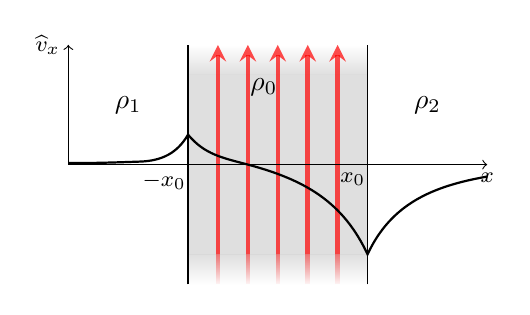
\begin{tikzpicture}[scale=0.76]
				\path [fill=lightgray, opacity=0.5] (2,-1.5) -- (2,1.5) -- (5,1.5) -- (5,-1.5) -- (2,-1.5);
				
				\shade[bottom color=white,top color=lightgray, opacity=0.5] (2,-2) to (5,-2) to (5,-1.5) to (2,-1.5) to (2,-2);
				
				\shade[top color=white,bottom color=lightgray, opacity=0.5] (2,2) to (5,2) to (5,1.5) to (2,1.5) to (2,2);
				
				\draw [-] (2,-2) -- (2,2);
				\draw [-] (5,-2) -- (5,2);
				
				\draw [ultra thick, red, -stealth,opacity=0.7] (2.5,-1.5) -- (2.5,2);
				\draw [ultra thick, red, path fading=south, opacity=0.5] (2.5,-2) -- (2.5,-1.5);
				\draw [ultra thick, red, -stealth,opacity=0.7] (3,-1.5) -- (3,2);
				\draw [ultra thick, red, path fading=south,opacity=0.5] (3,-2) -- (3,-1.5);
				\draw [ultra thick, red, -stealth,opacity=0.7] (3.5,-1.5) -- (3.5,2);
				\draw [ultra thick, red, path fading=south,opacity=0.5] (3.5,-2) -- (3.5,-1.5);
				\draw [ultra thick, red, -stealth,opacity=0.7] (4,-1.5) -- (4,2);
				\draw [ultra thick, red, path fading=south,opacity=0.5] (4,-2) -- (4,-1.5);
				\draw [ultra thick, red, -stealth,opacity=0.7] (4.5,-1.5) -- (4.5,2);
				\draw [ultra thick, red, path fading=south,opacity=0.5] (4.5,-2) -- (4.5,-1.5);
				
				\draw [thick] (0,0.025) to [out=0, in=-178] (1.2, 0.05) to [out=2, in=-120] (2,0.5) to [out=-50, in=165] (3,0) to [out=-15, in=115] (5,-1.5) to [out=65, in=-170] (7,-0.2);
				\draw [->] (0,0) -- (0,2);
				\draw [->] (0,0) -- (7,0);
				
				\node at (1,1) {$\rho_1$};
				\node at (6,1) {$\rho_2$};
				\node [right] at (2.88,1.3) {$\rho_0$};
				
				\footnotesize
				\node [below left] at (2.1,0) {$-x_0$};
				\node [below left] at (5.1,0) {$x_0$};
				
				\node [left] at (0,2) {$\widehat{v}_x$};
				\node [below] at (7,0) {$x$};
				\end{tikzpicture}
				\label{fig:surf quasi-saus}}}}
	%
	%
	\\
	%
	%
	\makebox[\textwidth][c]{
		\subfloat[Quasi-kink body mode]{\scalebox{1}{
				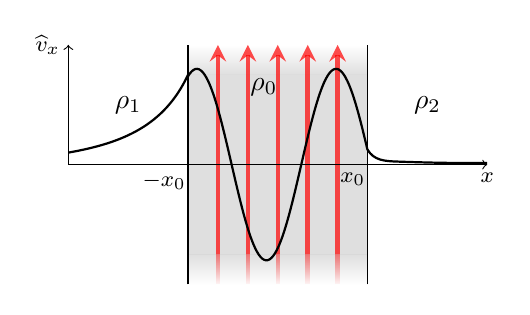
\begin{tikzpicture}[scale=0.76]
				\path [fill=lightgray, opacity=0.5] (2,-1.5) -- (2,1.5) -- (5,1.5) -- (5,-1.5) -- (2,-1.5);
				
				\shade[bottom color=white,top color=lightgray, opacity=0.5] (2,-2) to (5,-2) to (5,-1.5) to (2,-1.5) to (2,-2);
				
				\shade[top color=white,bottom color=lightgray, opacity=0.5] (2,2) to (5,2) to (5,1.5) to (2,1.5) to (2,2);
				
				\draw [-] (2,-2) -- (2,2);
				\draw [-] (5,-2) -- (5,2);
				
				\draw [thick] (7,0.025) to [out=180, in=358] (5.5, 0.05) to [out=178, in=300] (5,0.25);
				
				
				\draw [ultra thick, red, -stealth,opacity=0.7] (2.5,-1.5) -- (2.5,2);
				\draw [ultra thick, red, path fading=south, opacity=0.5] (2.5,-2) -- (2.5,-1.5);
				\draw [ultra thick, red, -stealth,opacity=0.7] (3,-1.5) -- (3,2);
				\draw [ultra thick, red, path fading=south,opacity=0.5] (3,-2) -- (3,-1.5);
				\draw [ultra thick, red, -stealth,opacity=0.7] (3.5,-1.5) -- (3.5,2);
				\draw [ultra thick, red, path fading=south,opacity=0.5] (3.5,-2) -- (3.5,-1.5);
				\draw [ultra thick, red, -stealth,opacity=0.7] (4,-1.5) -- (4,2);
				\draw [ultra thick, red, path fading=south,opacity=0.5] (4,-2) -- (4,-1.5);
				\draw [ultra thick, red, -stealth,opacity=0.7] (4.5,-1.5) -- (4.5,2);
				\draw [ultra thick, red, path fading=south,opacity=0.5] (4.5,-2) -- (4.5,-1.5);
				
				\draw [thick, smooth, samples=100, domain=2:5] plot (\x,{1.6*cos(2.7*(\x+0.18) r)});
				
				\draw [thick] (0,0.2) to [out=10, in=245] (2, 1.5);
				
				\draw [->] (0,0) -- (0,2);
				\draw [->] (0,0) -- (7,0);
				
				\node at (1,1) {$\rho_1$};
				\node at (6,1) {$\rho_2$};
				\node [right] at (2.88,1.3) {$\rho_0$};
				
				\footnotesize
				\node [below left] at (2.1,0) {$-x_0$};
				\node [below left] at (5.1,0) {$x_0$};
				
				\node [left] at (0,2) {$\widehat{v}_x$};
				\node [below] at (7,0) {$x$};
				\end{tikzpicture}
				\label{fig:body quasi-kink}}}
		%
		%
		%
		%
		\subfloat[Quasi-sausage body mode]{\scalebox{1}{
				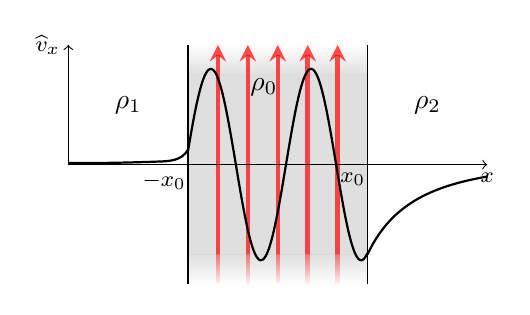
\begin{tikzpicture}[scale=0.76]
				\path [fill=lightgray, opacity=0.5] (2,-1.5) -- (2,1.5) -- (5,1.5) -- (5,-1.5) -- (2,-1.5);
				
				\shade[bottom color=white,top color=lightgray, opacity=0.5] (2,-2) to (5,-2) to (5,-1.5) to (2,-1.5) to (2,-2);
				
				\shade[top color=white,bottom color=lightgray, opacity=0.5] (2,2) to (5,2) to (5,1.5) to (2,1.5) to (2,2);
				
				\draw [-] (2,-2) -- (2,2);
				\draw [-] (5,-2) -- (5,2);
				
				\draw [thick] (0,0.025) to [out=0, in=-178] (1.5, 0.05) to [out=2, in=-120] (2,0.25);
				
				\draw [ultra thick, red, -stealth,opacity=0.7] (2.5,-1.5) -- (2.5,2);
				\draw [ultra thick, red, path fading=south, opacity=0.5] (2.5,-2) -- (2.5,-1.5);
				\draw [ultra thick, red, -stealth,opacity=0.7] (3,-1.5) -- (3,2);
				\draw [ultra thick, red, path fading=south,opacity=0.5] (3,-2) -- (3,-1.5);
				\draw [ultra thick, red, -stealth,opacity=0.7] (3.5,-1.5) -- (3.5,2);
				\draw [ultra thick, red, path fading=south,opacity=0.5] (3.5,-2) -- (3.5,-1.5);
				\draw [ultra thick, red, -stealth,opacity=0.7] (4,-1.5) -- (4,2);
				\draw [ultra thick, red, path fading=south,opacity=0.5] (4,-2) -- (4,-1.5);
				\draw [ultra thick, red, -stealth,opacity=0.7] (4.5,-1.5) -- (4.5,2);
				\draw [ultra thick, red, path fading=south,opacity=0.5] (4.5,-2) -- (4.5,-1.5);
				
				%\draw [thick] (2,0.5) to [out=-50, in=180] (2.3,0.25) to [out=0, in=180] (3.2,1) to [out=0, in=180] (4.1,0.1) to [out=-0, in=-120] (5,1.5);
				
				\draw [thick, smooth, samples=100, domain=2:5] plot (\x,{1.6*cos(3.75*(\x-0.705) r)});
				
				\draw [thick] (5,-1.5) to [out=65, in=-170] (7,-0.2);
				
				\draw [->] (0,0) -- (0,2);
				\draw [->] (0,0) -- (7,0);
				
				\node at (1,1) {$\rho_1$};
				\node at (6,1) {$\rho_2$};
				\node [right] at (2.88,1.3) {$\rho_0$};
				
				\footnotesize
				\node [below left] at (2.1,0) {$-x_0$};
				\node [below left] at (5.1,0) {$x_0$};
				
				\node [left] at (0,2) {$\widehat{v}_x$};
				\node [below] at (7,0) {$x$};
				\end{tikzpicture}
				\label{fig:body quasi-saus}}}}
	\caption{The transverse velocity perturbation amplitude, $\widehat{v}_x$ as a function of the transverse spatial coordinate, $x$, for quasi-sausage and quasi-kink modes in an isolated magnetic slab with external density ordering $\rho_1 > \rho_2$. \textcolor{red}{remove shading and arrows}}
\end{figure}


%------------------------------------------------------------------------------
\section{Asymmetric slab in a non-magnetic environment}
\label{sec: EVP non-mag}
%------------------------------------------------------------------------------

Much of the interesting physics due to waveguide asymmetry is exhibited by a magnetic slab with non-magnetic external plasma. We study this system in this Section.

By letting $B_1 = B_2 = 0$, the plasma in the asymmetric external regions is non-magnetic. Then the dispersion relation, Equation~\eqref{DR}, simplifies to
\begin{equation}
m_0^2\omega^4 + \frac{\rho_0}{\rho_1}m_1\frac{\rho_0}{\rho_2}m_2(\omega^2 - \omega_\textrm{A0}^2)^2 + m_0\omega^2(\omega^2 - \omega_{A0}^2)\left(\frac{\rho_0}{\rho_1}m_1 + \frac{\rho_0}{\rho_2}m_2\right)\coth{2m_0x_0} = 0, \label{DR non-mag}
\end{equation}
and the dispersion relation for a slab with first order asymmetry simplifies to
\begin{equation}
(\omega^2 - \omega_\textrm{A0}^2)\left(\frac{\rho_0}{\rho_1}m_1 + \frac{\rho_0}{\rho_2}m_2\right)  +  2\omega^2m_0\left(\begin{matrix}\tanh \\ \coth \end{matrix}\right)(m_0x_0) = 0. \label{DR approx non-mag}
\end{equation}


\subsection{Analytical solutions}
Analytical solutions to the dispersion relation can only be made under further assumptions about the plasma. In this section, incompressible (Section~\ref{sec: incomp}), zero-beta (Section~\ref{sec: zero-beta}), thin slab (Section~\ref{sec: thin slab}), and wide slab (Section~\ref{sec: wide slab}) approximations are explored. First, we deal with spurious solutions in Section~\ref{sec: spurious}.

\subsubsection{Spurious solutions} \label{sec: spurious}
There are three sets of spurious roots to the dispersion relation, $\omega = \pm kv_{A0}$, $\omega = \pm kc_0$, and $\omega = \pm kc_{T0}$. To treat these cases we refer back to the ODE for $\hat{v}_x(x)$ within the slab, Equation~\eqref{v_x ODE}.

When $\omega = \pm kc_{T0}$, $m_0$ is singular, in which case the solution to Equation~\eqref{v_x ODE} is $\hat{v}_x(x) = 0$ within the slab. From Equation\eqref{mom z 2}, it follows that $\hat{v}_z \propto \hat{v}_x'$, we therefore also have $\hat{v}_z(x) = 0$. Given that we are assuming ideal plasma so that the magnetic flux is frozen to the plasma, this means that there is no magnetic field perturbation either. Therefore, $\omega = \pm kc_{T0}$ is a spurious solution.

\textcolor{red}{edit from below here on spurious sols.}

When $\omega = \pm kc_0$, we have $m_0 = 0$, therefore Equation~\eqref{v_x ODE} has general solution $\hat{v}_x(x) = Bx + C$ for constants $B$ and $C$. Equation~\eqref{mom z 2} further shows that  $\hat{v}_x' = 0$. Therefore, $B = 0$ and $\hat{v}_x(x) = C$. The $z$-component of Equation~\eqref{ind eqn lin} tells us that $\hat{b}_z \propto \hat{v}_x'$ and so $\hat{b}_z = 0$, therefore the magnetic pressure perturbation is zero. It can be shown that the plasma pressure is
\begin{equation}
\hat{p}(x) = - \frac{i\rho_0c_0^2}{\omega}\left[\frac{Cx(k^2v_A^2 - \omega^2)}{c_0^2} + C_2\right],
\end{equation}
within the slab, for constant $C_2$. To make pressure balance over each interface we must have $C=0$. This means that $v_x(x)=0$ within the slab and therefore across the whole domain. Therefore the pressure outside the slab is zero (since it is proportional to $\hat{v}_x' = 0$) , and by matching pressure, it is zero within the slab. Therefore this solution is a trivial wave. (is this the entropy wave???)

On the other hand, when $\omega = kv_A$, the total pressure amplitude, $\hat{P}(x)$, is such that
\begin{equation}
\widehat{P}(x)=\widehat{v}_x'(x)
\begin{cases}
\Lambda_1/m_1, & \text{if } x<-x_0, \\
\Lambda_0/m_0, & \text{if }|x|\leq{}x_0, \\
\Lambda_2/m_2, & \text{if }x>x_0,
\end{cases}
\end{equation}
where
\begin{equation}
\Lambda_0=-\frac{i\rho_0(k^2v_\textrm{A}^2-\omega^2)}{m_0\omega}, \quad \Lambda_1=\frac{i\rho_1\omega}{m_1}, \quad \text{and} \quad \Lambda_2=\frac{i\rho_2\omega}{m_2}. \label{Lambdas}
\end{equation}
(the derivation for this still holds). Note that the singularity due to the division by $m_0^2$ is regulated by the factor of $k^2v_A^2 - \omega^2$ in $\Lambda_0$. Therefore, since $\hat{v}_x' = B$ is constant in the slab, then so is $\hat{P}$. When we match the total pressure over the boundaries we find that the slab must be symmetric. Therefore $B=0$ to ensure that the velocity profile is symmetric. Therefore $\hat{v}_x' = B = 0$, so there is no pressure perturbation. In particular, there is no pressure perturbation outside the slab, which implies that there is no velocity perturbation outside the slab, because they both depend on the same constants. Therefore by continuity of velocity and the fact that it is constant within the slab, the velocity perturbation is zero everywhere. Therefore there is no wave.


\subsubsection{Limiting case - incompressible plasma} \label{sec: incomp}

Compressibility is essential for the propagation of sound waves. Consider the dispersion relation, Equation~\eqref{DR non-mag}, in the limit of incompressibility, that is, when $\gamma \to \infty$. In this limit, the sound speeds become unbounded and the tube speed in the slab behaves like $c_{T0} \to {v_{A0}}$. This means that $m_j \to {k}$ for $j = 0, 1, 2$, so that the dispersion relation reduces to
\begin{equation}
\omega^4 + \frac{\rho_0^2}{\rho_1\rho_2}(\omega^2 - \omega_{A0}^2)^2 + \omega^2(\omega^2 - \omega_{A0}^2)\left(\frac{\rho_0}{\rho_1} + \frac{\rho_0}{\rho_2}\right) \coth{2kx_0} = 0. \label{DR incomp}
\end{equation}
This is a special case of the dispersion relation previously derived by \cite{rud92}, who found solitons propagating on a system of $N$ tangential discontinuities. Equation~\eqref{DR incomp} is a quadratic equation in $\omega^2$ which has solutions
\begin{equation}
\omega^2 = k^2v_{A0}^2\left(\frac{2 + \sigma \pm \sqrt{\sigma^2 - 4\frac{\rho_1\rho_2}{\rho_0^2}}}{1 + \sigma + \frac{\rho_1\rho_2}{\rho_0^2}}\right),
\end{equation}
where
\begin{equation}
\sigma = \left(\frac{\rho_1}{\rho_0} + \frac{\rho_2}{\rho_0}\right)\coth{2kx_0}.
\end{equation}
These solutions hold for all $kx_0 > 0$ and describe surface modes with sub-Alfv\'enic phase speed. The solution found by the plus (minus) on the numerator is the sausage (kink) eigenfrequency.

Figures~\ref{fig:incomp22}-\ref{fig:incomp10001} demonstrate that in a thin ($kx_0 \ll 1$) incompressible slab, the phase speeds of these modes approach zero or the Alfv\'{e}n speed. In a symmetric wide incompressible slab, the phase speeds converge to the same speed (Figure~\ref{fig:incomp22}), whereas in an asymmetric slab, the phase speeds converge to different speeds (Figures~\ref{fig:incomp102}-\ref{fig:incomp10001}) that depend upon the values of the external densities. This observation is mirrored by both fast and slow surface modes in the more general solutions of a compressible slab solved numerically to give Figure~\ref{fig:slow modes density}.

\begin{figure}
	\centering
	\subfloat[$\rho_1/\rho_0=2$, $\rho_2/\rho_0=2$]{\includegraphics[scale=0.45]{\figdir Incomp_2_2.pdf}
		\label{fig:incomp22}}
	\subfloat[$\rho_1/\rho_0=10$, $\rho_2/\rho_0=2$]{\includegraphics[scale=0.45]{\figdir Incomp_10_2.pdf}
		\label{fig:incomp102}} \\
	\subfloat[$\rho_1/\rho_0=10$, $\rho_2/\rho_0=0.1$]{\includegraphics[scale=0.45]{\figdir Incomp_10_01.pdf}
		\label{fig:incomp1001}}
	\subfloat[$\rho_1/\rho_0=100$, $\rho_2/\rho_0=0.1$]{\includegraphics[scale=0.45]{\figdir Incomp_100_01.pdf}
		\label{fig:incomp10001}}
	\caption{The behaviour of the modes in an incompressible slab. The fast surface modes and all the body modes degenerate leaving two sub-Alfv\'{e}nic surface modes. (a) A symmetric slab, (b)-(d) asymmetric slabs.}
\end{figure}


\subsubsection{Limiting case - low-beta} \label{sec: zero-beta}

The case when the magnetic pressure strongly dominates the gas pressure within the slab, \textit{i.e.} $\beta := 2\mu_0{p_0}/B_0^2 \ll 1$, is known as the \textit{low-beta approximation}. This approximation is equivalent to the Alfv\'{e}n speed dominating the sound speed in the slab and provides a good approximation of the solar coronal environment. In this section, the results are to quadratic order in $\beta$.

Under this speed ordering, $m_0^2\approx{}k^2-\omega^2/v_\textrm{A}^2$. After a numerical investigation, it is clear that the frequency of waves in this approximation satisfies $\omega^2\ll{}k^2v_\textrm{A}^2$, in which case $m_0^2\approx k^2$ provides a valid approximation. This means that $m_0^2>0$ and the solutions are surface modes. For a symmetric slab of low-beta plasma (\textit{e.g.} \citealt{rob81b}), the dispersion relation reduces to a quadratic expression in $\omega^2$ whose solutions are the fast sausage and kink surface modes given by
\begin{equation}
\omega^2=k^2c_\textrm{e}^2\left(\frac{\sqrt{1+\gamma^2\left(\hspace{-0.11in}\begin{matrix}&\tanh^2 \\&\coth^2 \end{matrix}\right)(kx_0)}-1}{\frac{1}{2}\gamma^2\left(\hspace{-0.11in}\begin{matrix}&\tanh^2 \\&\coth^2 \end{matrix}\right)(kx_0)}\right),
\end{equation}
where $c_\textrm{e}$ is the external sound speed, along with a spurious solution.

Unfortunately, for the more general case of an asymmetric slab of low-beta plasma, the dispersion relation does not reduce to an analytically solvable equation. However, we find numerically that there are two fast surface modes. The quasi-sausage surface mode is not present for small $kx_0$, but becomes a solution at an intermediate value of $kx_0$ with phase speed $\omega^2/k^2=\min{(c_1^2,c_2^2)}$. The quasi-kink surface mode is present for all values of $kx_0$. Qualitatively, the solutions for a low-beta plasma are analogous to the fast quasi-sausage and quasi-kink mode solutions, discussed later in Sections~\ref{sec:thin} and~\ref{sec:wide}.

In the following section, thin and wide slab approximations are made to the approximate dispersion relation, Equation~\eqref{DR approx}, rather than the exact dispersion relation, Equation~\eqref{DR}. Here, the aim is to retrieve the variety of wave modes with future applications in mind.


\subsubsection{Limiting case - thin slab} \label{sec: thin slab}

Consider the case where the wavelength, $\lambda$, is much greater than the width of the slab, $2x_0$, \textit{i.e} $2x_0/\lambda = kx_0/\pi \ll 1$, or equivalently $kx_0 \ll 1$.

First, consider the quasi-sausage surface modes, which are governed by the $\tanh$ version of Equation~\eqref{DR approx non-mag}, for $m_0^2 > 0$. In the thin slab limit, this equation reduces to
\begin{equation}
(\omega^2 - \omega_\textrm{A0}^2)\left(\frac{\rho_0}{\rho_1}m_1 + \frac{\rho_0}{\rho_2}m_2\right) -  2\omega^2m_0^2x_0 = 0. \label{thin}
\end{equation}
Clearly, $\omega^2={k^2v_\textrm{A}^2}$ is a solution, but as noted in Section~\ref{sec: spurious}, it is spurious. The other solution for $\omega^2$ behaves like $\omega^2 \to k^2c_\textrm{T0}^2$ as $kx_0 \to 0$. To first order in $kx_0$, this solution is a slow quasi-sausage surface mode given by
\begin{equation}
\omega^2 = k^2c_\textrm{T0}^2 \left[1 - \frac{2(kx_0)(c_0^2 - c_\textrm{T0}^2)}{(c_0^2 + v_\textrm{A0}^2)\left(\frac{\rho_0}{\rho_1}\frac{\sqrt{c_1^2 - c_\textrm{T0}^2}}{c_1} + \frac{\rho_0}{\rho_2}\frac{\sqrt{c_2^2 - c_\textrm{T}^2}}{c_2}\right)}\right],
\label{thin slab slow saus surf}
\end{equation}
which is less than $k^2c_\textrm{T0}^2$ and exists only when $c_1 > c_\textrm{T0}$ and $c_2 > c_\textrm{T0}$. 

It is interesting to note that if $c_1 = c_2 = c_\textrm{e}$ (and therefore $\rho_1 = \rho_2 = \rho_\textrm{e}$ by Equation~\eqref{sound and density}), then there exists a second solution to Equation~\eqref{thin}. By letting $\omega^2 = k^2c_\textrm{e}^2(1 + \nu)$ for some $\nu \ll 1$ in Equation~\eqref{thin}, we find the solution to be
\begin{equation}
\omega^2 = k^2c_\textrm{e}^2\left(1 - \left[\frac{\rho_\textrm{e}}{\rho_0}\frac{c_\textrm{e}^2(c_0^2 - c_\textrm{e}^2)(kx_0)}{(c_0^2 + v_\textrm{A0}^2)(c_\textrm{T0}^2 - c_\textrm{e}^2)}\right]^2\right)
\label{thin slab fast saus surf}
\end{equation}
in the thin slab limit. This is a fast sausage surface mode, and it degenerates (as a solution in the thin slab limit) as $c_1$ and $c_2$ become distinct. This mode can still exist with a phase speed below the cut-off at $\min(c_1, c_2)$ (see Section~\ref{sec: disp diagrams}).

Next, consider quasi-kink surface mode solutions in the thin slab limit, which are governed by the $\coth$ version of Equation~\eqref{DR approx non-mag}, for $m_0^2 > 0$. As $kx_0 \to 0$, we have $m_0x_0 \to 0$, so $\coth{m_0x_0} \to 1/m_0x_0$. This simplifies the dispersion relation to
\begin{equation}
\omega^2 = \frac{k^2x_0v_\textrm{A0}^2\left(\frac{\rho_0}{\rho_1}m_1 + \frac{\rho_0}{\rho_2}m_2\right)}{\left(\frac{\rho_0}{\rho_1}m_1x_0 + \frac{\rho_0}{\rho_2}m_2x_0\right) + 2} \approx \frac{1}{2}k^2v_\textrm{A0}^2\left(\frac{\rho_0}{\rho_1} + \frac{\rho_0}{\rho_2}\right)kx_0.
\label{thin slab slow kink surf}
\end{equation}
This is a slow quasi-kink surface mode that behaves like $\omega/k \to 0$ in the thin slab limit.

For body waves in the thin slab approximation, following the same procedure as for surface waves turns out to be fruitless, so we must reconsider our assumptions. Unfortunately, letting $m_0x_0 \to 0$ as $kx_0 \to 0$, whilst valid for surface modes, is not valid for body modes. Instead, we must consider the scenario where $m_0x_0$ remains finite as $kx_0 \to 0$. This can occur only if $|m_0^2| \to \infty$ as $kx_0 \to 0$.  To ensure that $|m_0^2| \to \infty$, we are restricted to solutions that behave like $\omega^2 \to k^2c_\textrm{T0}^2$ as $kx_0 \to 0$. Considering Equation~\eqref{DR approx non-mag}, this can only be the case when $m_0^2 < 0$, \textit{i.e.} only for body modes. To find these solutions, set $\omega^2 = k^2c_\textrm{T0}^2(1 + \nu(kx_0)^2)$ for some $\nu > 0$ that is to be determined. To see why this form has been chosen, a substitution into the definition of $m_0^2$ demonstrates that $|m_0^2| \to \infty$ and $m_0x_0$ remains bounded as $kx_0 \to 0$, as required. Using this ansatz, Equation~\eqref{DR approx} has a countably infinite set of quasi-sausage body solutions which, in the thin slab limit, behave like
\begin{equation}
\omega^2 = k^2c_\textrm{T0}^2\left[1 + \frac{c_\textrm{T0}^4(kx_0)^2}{c_0^2v_\textrm{A0}^2\pi^2j^2}\right], \quad \text{for} \quad j = 1, 2, \ldots. \label{thin slab saus body}
\end{equation}
There are also quasi-kink body solutions that, in the thin slab limit, behave like
\begin{equation}
\omega^2 = k^2c_\textrm{T0}^2\left[1 + \frac{c_\textrm{T0}^4(kx_0)^2}{c_0^2v_\textrm{A0}^2\pi^2(j - \frac{1}{2})^2}\right], \quad \text{for} \quad j = 1, 2, \ldots. \label{thin slab kink body}
\end{equation}
Equations~\eqref{thin slab saus body} and \eqref{thin slab kink body} show us that to quadratic order in $kx_0$ the quasi-sausage and quasi-kink body modes do not depend on the external environment parameters. The effects of external density and temperature are felt in the higher order terms, which explains why Equations~\eqref{thin slab saus body} and~\eqref{thin slab saus body} are identical to the corresponding solutions in a thin symmetric slab derived by \citealt{rob81b}. This also explains theoretically why body modes only weakly depend on the asymmetry of the external plasma, as discussed in the context of magnetic field diagnostics in Section~\ref{sec: SMS}.


\subsubsection{Limiting case - wide slab} \label{sec: wide slab}

The wide slab approximation the limit of the slab width being is much larger than the wavelength, \textit{i.e.} when $kx_0 \gg 1$. To understand the properties of the eigenfrequencies in a wide asymmetric slab, it is instructive to return to the dispersion relation in lambda notation, Equation~\eqref{DR lambda}. For surface modes in the slab, the wide slab approximation implies that $m_0x_0 \gg 1$, therefore $\coth{m_0x_0} \approx 1$ (this is checked \textit{a posteriori} by \cite{rob81b}). Under this approximation, Equation~\eqref{DR lambda}, becomes
\begin{equation}
(\Lambda_0 + \Lambda_1)(\Lambda_0 + \Lambda_2) = 0,
\end{equation}
which gives us two families of solutions, one satisfying $\Lambda_0 + \Lambda_1 = 0$ and the other satisfying $\Lambda_0 + \Lambda_2 = 0$. These are equivalent to
\begin{equation}
	\rho_0m_j(\omega^2 - \omega_\textrm{A0}^2) + \rho_jm_0\omega^2 = 0,
\end{equation}
for $j = 1, 2$, respectively. This equation is the same as the dispersion relation governing surface waves along a single interface between a magnetized and a non-magnetized plasma, Equation\eqref{DR interface} for $v_{A1} = v_{A2} = 0$. Hence, the surface mode solutions of a wide asymmetric slab are precisely the those that propagate along each interface independently. This corroborates our intuition that, as the slab width increases, the interfaces have diminishing influence on each other. In the wide slab limit, the interfaces have no influence on each other at all, allowing each to oscillate independently with its own characteristic frequency.

Unfortunately, the body waves have no parallel in the single interface model because body waves in a slab owe their existence to both of the two interfaces. In the wide slab limit, body waves behave like $\omega^2 \to k^2c_0^2$ as $kx_0 \to \infty$. To see this, substitute the ansatz $\omega^2 = k^2c_0^2 \left(1 + \nu/(kx_0)^2\right)$ into the dispersion relation, Equation~\eqref{DR approx non-mag}, to retrieve the family of quasi-sausage body modes given by
\begin{equation}
\omega^2 = k^2c_0^2\left[1 - \frac{\pi^2(j - \frac{1}{2})^2c_0^2}{(v_{A0}^2 - c_0^2)(kx_0)^2}\right], \quad j = 1, 2, \ldots \label{wide slab saus body}
\end{equation}
in the wide slab limit. Similarly, there exist quasi-kink body modes given by
\begin{equation}
\omega^2 = k^2c_0^2\left[1 - \frac{\pi^2j^2c_0^2}{(v_{A0}^2 - c_0^2)(kx_0)^2}\right], \quad j = 1, 2, \ldots \label{wide slab kink body}
\end{equation}
in the wide slab limit. These solutions are valid only when $v_{A0} > c_0$.

This analysis may be repeated for $v_{A0} < c_0$ to find that, in the wide slab limit, there exist quasi-sausage body modes given by
\begin{equation}
\omega^2 = k^2v_\textrm{A0}^2\left[1 - \frac{\pi^2(j - \frac{1}{2})^2v_{A0}^2}{(c_0^2 - v_{A0}^2)(kx_0)^2}\right], \quad \text{for} \quad j = 1, 2, \ldots \label{wide slab saus body2}
\end{equation}
and quasi-kink body modes of the form
\begin{equation}
\omega^2 = k^2v_{A0}^2\left[1 - \frac{\pi^2j^2v_\textrm{A0}^2}{(c_0^2 - v_{A0}^2)(kx_0)^2}\right], \quad \text{for} \quad j = 1, 2, \ldots . \label{wide slab kink body2}
\end{equation}
These solutions demonstrate that, to quadratic order in $1/kx_0$, the wide slab body modes are independent of the external plasma parameters. Therefore, Equations~\eqref{wide slab saus body}-\eqref{wide slab kink body2} are identical to the body mode solutions in a wide symmetric slab \citep{rob81b}. Equations~\eqref{thin slab slow saus surf}-\eqref{thin slab kink body},~\eqref{wide slab saus body} and~\eqref{wide slab kink body} also appear in~\cite{li_etal13} for a symmetric magnetic slab with shear flow when the shear flow speed is set to zero.


\subsection{Numerical solutions} \label{sec: numerical solutions}

Numerical methods are required to investigate solutions to the asymmetric slab dispersion relation, Equation~\eqref{DR non-mag}, without having to rely on further approximations. Focus is placed on the additional physics that arises from the asymmetry of the external plasma.


\subsubsection{Description of numerical procedure}
To solve Equation~\eqref{DR non-mag} numerically, we view the left-hand-side as a function $D(\omega)$ of the wave frequency, $\omega$, and wavenumber $k$. We call this function a \textit{dispersion function}. This means that for a given wavenumber value, we are solving a simple root-finding problem, where the aim is to find the zeros of the dispersion function, \textit{i.e.} $\omega$ such that $D(\omega) = 0$. To accomplish this, we use the \textit{secant method}. The Secant method is a standard root-finding procedure that is equivalent to the Newton-Raphson method utilising a finite difference approximation to the derivative of the dispersion function. this is chosen because the derivative of the dispersion function is not easily found and there is only a small trade-off with algorithmic efficiency\footnote{The order of convergence of the Newton-Raphson method is 2 and whereas the order of convergence of the secant method is the golden ratio, $\psi \approx 1.618$.}.


\subsubsection{Dispersion diagrams} \label{sec: disp diagrams}

\begin{figure}[]
	\centering
	\subfloat[$v_{A0} > c_0$]{\includegraphics[scale=0.45]{\figdir disp_sbs_R1-5.pdf}
		\label{fig: disp sbs}}
	\subfloat[$v_{A0} < c_0$]{\includegraphics[scale=0.45]{\figdir disp_sbb_R1-5.pdf}
		\label{fig: disp sbb}}
	\caption{Dispersion diagram for the dispersion relation, Equation~\eqref{DR non-mag}. The surface (body) modes are in plotted red (blue) and the sausage (kink) modes are represented by solid (dashed) lines. The density ratios are $\rho_1/\rho_0 = 1.5$ and $\rho_2/\rho_0 = 2$, and the characteristic speed orderings are $c_2 = 1.2c_0$ and (a)$v_{A0} = 1.3c_0$ and (b)$v_{A0} = 0.9c_0$.}
	\label{fig: disp}
\end{figure}

Figure~\ref{fig: disp} illustrates the solutions to the dispersion relation, Equation~\eqref{DR non-mag}, for two orderings of the characteristic speeds. Figure~\ref{fig: disp sbs} illustrates the spectrum of modes we would expect to find in the corona and Figure~\ref{fig: disp sbb} illustrates the spectrum of modes we would expect to find in the photosphere.

In both coronal and photospheric conditions, there are slow sausage and kink surface modes (illustrated by the slowest red solution lines) and an infinite sequence of slow sausage and kink body modes (illustrated by the slowest blue solution lines). Each sausage body mode propagates faster than its corresponding kink mode, which agrees with the analytical solutions in Equations~\eqref{thin slab saus body},~\eqref{thin slab kink body},~\eqref{wide slab saus body}-\eqref{wide slab kink body2}.

In coronal conditions, there exist fast sausage and kink surface modes with phase speeds between $c_0$ and $\min{c_1, c_2}$. Figure~\ref{fig: disp sbs} shows that the minimum of $c_1$ and $c_2$ becomes a new cut-off, causing the fast kink surface mode to transform into a slow kink first-order body mode for smaller values of the slab width\footnote{More precisely, the non-dimensionalised slab half-width.}, $kx_0$. In Section~\ref{sec: critical slab width}, the precise value of this critical slab width is determined and the eigenfunction is analysed across this transition.

In photospheric conditions, there exists an infinite sequence of fast sausage and kink body modes with phase speeds between $c_0$ and $\min{c_1, c_2}$. For values of the slab width below a cut-off value (that is unique for every order of body mode), these modes cease to be trapped by the slab and leak energy into the surrounding plasma. In Section~\ref{sec: fast mode cut-off}, the precise value of these cut-off values is determined.


\subsubsection{Critical slab width for kink mode transformation} \label{sec: critical slab width}
First, let's derive an analytical expression for the critical slab width, over which the slow kink first-order body mode transitions into a fast kink surface mode. To do this, let $\omega^2 = k^2c_0^2(1 + \nu)$ for some $\nu \ll 1$. Then we have
\begin{equation}
m_0^2 = -\frac{\nu k^2c_0^2(v_A^2 - c_0^2(1 + \nu))}{(c_0^2 + v_A^2)(c_T^2 - c_0^2(1 + \nu))},
\end{equation}
which, when terms of quadratic and higher order in $\nu$ are neglected, reduces to
\begin{equation}
m_0^2 = \frac{\nu k^2(v_A^2 - c_0^2)}{c_0^2},
\end{equation}
and therefore,
\begin{equation}
\tanh(2m_0x_0) = 2kx_0\sqrt{\frac{\nu(v_A^2 - c_0^2)}{c_0^2}}.
\end{equation}
Substituting these into the dispersion relation for quasi-kink modes, neglecting terms of quadratic and higher order in $\nu$, and solving for $kx_0$ gives us the critical value for the 1st fast kink body mode as
\begin{equation}
kx_0 = \frac{c_0^2 \left(\frac{\rho_2}{\rho_0}c_2\sqrt{c_1^2 - c_0^2} + \frac{\rho_1}{\rho_0}c_1\sqrt{c_2^2 - c_0^2}\right)}{2(v_A^2 - c_0^2)\sqrt{(c_1^2 - c_0^2)(c_2^2 - c_0^2)}}.
\end{equation}

Across this transitional value, the eigenfunction changes functional form inside the slab from a trigonometric to a hyperbolic function (see Figure~\ref{fig: transitional kink eigenfunction}). 
\begin{figure}
	\centering
	\includegraphics[width=\textwidth]{\figdir xi_of_x_body_surface_conversion.png}
	\caption{The eigenfunction of the transitional kink mode. The critical slab width occurs between $kx_0 = 4$ and $kx_0 = 5$.}
	\label{fig: transitional kink eigenfunction}
\end{figure}


\subsubsection{Fast mode cut-off} \label{sec: fast mode cut-off}
If $c_1 = c_2$, we have a symmetric slab and therefore no fast mode cut-off. Let $c_1 \neq c_2$ and let $\omega = \min(kc_1, kc_2)$. Without loss of generality, consider the case where $c_1 < c_2$ so that $m_1 = 0$. Therefore,
\begin{equation}
m_0^2 = \frac{k^2 (c_0^2 - c_1^2)(v_A^2 - c_1^2)}{(c_0^2 + v_A^2)(c_T^2 - c_1^2)} = k^2m^2,
\quad \text{and} \quad
m_2^2 = k^2\left(1-\frac{c_1^2}{c_2^2}\right).
\end{equation}
Substituting these expressions in the dispersion relation and solving for $kx_0$ gives the fast mode cut-off values
\begin{equation}
kx_0 = \frac{1}{2m} \tanh^{-1}\left( \frac{1}{m c_1^2} \frac{\rho_0}{\rho_2} \sqrt{1 - \frac{c_1^2}{c_2^2}}(c_1^2 - v_{A0}^2) \right). \label{fast mode cut-off}
\end{equation}

For surface modes, $m_0^2 > 0$, therefore the argument of the $\tanh^{-1}$ term is real, so that Equation~\eqref{fast mode cut-off} admits a single solution. This corresponds to the cut-off value for the fast sausage surface mode in Figure~\ref{fig: disp sbs}.
 
For body modes, $m_0^2 < 0$, therefore the argument of the $\tanh^{-1}$ term is imaginary. Defining $n \in \mathbb{R}$ as $n = im$ and utilising the fact that $\tanh^{-1}(ix) = i\tan^{-1}(x)$, we can rewrite Equation~\eqref{fast mode cut-off} as
\begin{equation}
kx_0 = \frac{1}{2n} \left[\tan_p^{-1}\left( \frac{1}{n c_1^2} \frac{\rho_0}{\rho_2} \sqrt{1 - \frac{c_1^2}{c_2^2}}(v_{A0}^2 - c_1^2) \right) + j\pi \right], \label{fast mode cut-off 2}
\end{equation}
for $j \in \mathbb{Z}$ and $\tan_p^{-1}$ refers to the principle value of the inverse $\tan$ function, \textit{i.e.} the value in the range $(-\pi/2, \pi/2)$. This infinite set of solutions corresponds to the infinite set of fast sausage and kink body modes, each of which has a cut-off, as seen in Figure~\ref{fig: disp sbb}.

When the slab is symmetric, the cut-off for both the fast sausage surface mode and the fast sausage first-order body mode are zero. See this by setting $c_1 = c_2$ in the argument of $\tanh^{-1}$ and $\tan_p^{-1}$ in Equations~\eqref{fast mode cut-off} and~\eqref{fast mode cut-off 2}, respectively. This means that the modes cease to have a cut-off at all and exist for all values of the slab width, $kx_0$, which corroborates with the results of \cite{rob81b}.


\subsubsection{Varying the degree of asymmetry}

\begin{figure}
	\centering
	\subfloat[]{\includegraphics[scale=0.5]{\figdir SS_SK_DS_v2.pdf}
		\label{fig: density ratio}} \\
	%\vspace{-0.4in}
	\subfloat[$\frac{\rho_\textrm{e}}{\rho_0}=0.1$]{\includegraphics[scale=0.45]{\figdir SS_SK_Re01_v2.pdf}
		\label{fig: density ratio 0.1}}
	\subfloat[$\frac{\rho_\textrm{e}}{\rho_0}=10$]{\includegraphics[scale=0.45]{\figdir SS_SK_Re10_v2.pdf}
		\label{fig: density ratio 10}}
	\caption{The effect of varying the ratio, $\rho_\textrm{e}/\rho_0$, of the slab density to the symmetric external density, on the dispersion of the slow surface modes of a magnetic slab in a symmetric external plasma. The red and blue surfaces correspond to the kink and sausage modes, respectively. Panels (b) and (c) are slices of panel (a) at specific values of $\rho_\textrm{e}/\rho_0$. These slices are superimposed onto panel (a) as black lines. The characteristic speed orderings are $v_\textrm{A0} = 0.5c_0$, $c_\textrm{e} = c_0$.}
\end{figure}


\begin{figure}
	\centering
	\subfloat[]{\includegraphics[scale=0.5]{\figdir FullDR_SS_SK_DS_v2.pdf}
		\label{fig: slow modes density}} \\
	\subfloat[$kx_0 = 0.01$]{\includegraphics[scale=0.45]{\figdir FullDR_SS_SK_Kfixed001_v2.pdf}
		\label{fig: slow modes density 0.01}}
	\subfloat[$kx_0 = 0.1$]{\includegraphics[scale=0.45]{\figdir FullDR_SS_SK_Kfixed01_v2.pdf}
		\label{fig:slow modes density 0.1}} \\
	\subfloat[$kx_0 = 1$]{\includegraphics[scale=0.45]{\figdir FullDR_SS_SK_Kfixed1_v2.pdf}
		\label{fig: slow modes density 1}}
	\subfloat[$kx_0 = 3$]{\includegraphics[scale=0.45]{\figdir FullDR_SS_SK_Kfixed3_v2.pdf}
		\label{fig: slow modes density 3}}
	\caption{(a) The slow quasi-sausage (blue) and quasi-kink (red) surface mode solutions of the dispersion relation (Equation~\eqref{DR}) are plotted showing the variation of the dispersion as the ratio of one external density to the internal density is changed. The other density ratio is held fixed at $\rho_2/\rho_0=2$. The characteristic speed orderings are $c_2=0.7c_0$, $v_\textrm{A}=0.4c_0$, and $c_1$ varies to satisfy equilibrium pressure balance, given by Equation~\eqref{sound and density}. Panels (b)-(e) are slices of panel (a) for specific values of the non-dimensional slab width, $kx_0$.}
\end{figure}


First, consider a magnetised slab with symmetric non-magnetic external plasma, as described by \cite{rob81b} and summarised in Section~\ref{sec: MHD waves sym slab}. Figures~\ref{fig: density ratio}-\ref{fig: density ratio 10} illustrate how varying the ratio of external to internal density affects the propagation speeds of the slow kink and sausage surface modes. An increase in the density ratio, $\rho_\textrm{e}/\rho_0$, causes a decrease in the propagation speed of the slow modes. The fast surface modes demonstrate an identical behaviour (not shown). The body modes are weakly dependent on the external density, so that the propagation speed decreases only negligibly as the density ratio increases.

More generally, consider an asymmetric slab whose equilibrium conditions are given by Figure~\ref{fig: eq}. Figures~\ref{fig: slow modes density}-\ref{fig: slow modes density 3} illustrate the behaviour of the slow surface modes as the external density on one side of the slab is varied while holding fixed the other external density. The slice where $\rho_1/\rho_0 = 2$ corresponds to a symmetric slab, where the usual behaviour is observed: that the phase speed of the two slow surface modes converges to a speed that is slower than the tube speed, $c_\textrm{T0}$, as the slab width increases. However, as the external densities become distinct, the phase speeds of these modes no longer converge to the same value in the wide slab limit. This can also be seen in Figures~\ref{fig: disp sbs} and~\ref{fig: disp sbb}.

For a wide slab width, $kx_0 \gg 1$, Figure~\ref{fig: slow modes density 3} illustrates that the eigencurves of the slow surface modes possess a wave phenomenon known as \textit{avoided crossing}. Avoided crossings occur when the phase speeds of two wave modes avoid intersecting when a parameter of the system is varied. This occurs when there are constraints preventing two solution from being equal and it demonstrates a transferral of properties between the two modes. Analysis this phenomenon can be used to give insight into the modal structure. There is rich literature regarding avoided crossings for the eigensolutions of a wide range of physical processes including coupled spring oscillations in classical mechanics \citep{nov10} and energy level repulsion in quantum physics \citep{naq_etal72}. In MHD wave theory, the subject has been covered only briefly, for example, between fast and slow magneto-acoustic gravity waves in a magnetically stratified plasma by \cite{abd90} and \cite{mat_etal2016}.

\begin{figure} []
	\centering
	\subfloat[]{\includegraphics[scale=0.5]{\figdir disp.pdf}
		\label{fig: disp avoided crossing}} \\
	\makebox[\textwidth][c]{
		\subfloat[]{\includegraphics[scale=0.47]{\figdir xix_v2.pdf}
			\label{fig: xi}}}
	\caption{(a) The slow surface mode solutions of the dispersion relation, Equation~\eqref{DR}, are plotted showing the variation of the dispersion as the ratio of one external density to the internal density is changed. The other density ratio is held fixed at $\rho_2/\rho_0=2$ and the non-dimensionalised slab width $kx_0 = 1.5$. The characteristic speed orderings are $c_2=0.7c_0$, $v_\textrm{A}=0.4c_0$, and $c_1$ varies to satisfy equilibrium pressure balance, given by Equation~\eqref{sound and density}. The parameters at each blue and red dot in panel(a) are used to plot the spatial variation of the transverse displacement perturbation, $\widehat{\xi}_x$, given by panel (b). The upper (lower) plots in panel (b) correspond to the quasi-sausage (quasi-kink) mode solutions.}
	\label{fig: avoided crossing}
\end{figure}

\begin{figure}
	\centering
	\includegraphics[width=\textwidth]{\figdir xi_of_x_slow_body.png}
	\caption{The variation (or lack thereof) of the first three slow sausage and kink body eigenfunctions as the asymmetry in the background plasma is varied. The first, third, and fifth rows are kink modes and the second, fourth, and sixth rows are sausage modes. The density ratio $\rho_1/\rho_0$ is varied while the other density ratio is held fixed at $\rho_2/\rho_0 = 2.0$. The middle column of panels for which $\rho_1/\rho_0 = 2.0$ corresponds to a symmetric slab.}
	\label{fig: body eigenmodes}
\end{figure}

In the present study, the avoided crossing occurs between quasi-kink and quasi-sausage surface solutions to the asymmetric slab. This explains why the dispersion relation does not decouple into two equations (Section~\ref{sec: symmetric comp}). Figure~\ref{fig: avoided crossing} demonstrates that during the transition across the avoided crossing, the quasi-sausage and quasi-kink modes exchange the slab boundary upon which the largest perturbation occurs. For example, the left plots of Figure~\ref{fig: xi} show that the quasi-sausage mode has its highest amplitude on the interface of highest local phase-speed (equivalently, lowest external density). The quasi-kink mode demonstrates the opposite behaviour. The central plots show the special case of a symmetric slab, where $\rho_1 = \rho_2$, demonstrating the spatial antisymmetry and symmetry in the symmetric sausage and kink mode, respectively. As the left external density, $\rho_1$, dominates the right external density, $\rho_2$, the right plots of Figure~\ref{fig: xi} show that, again, the quasi-sausage mode has its higher amplitude on the interface of higher local phase-speed, but this is now on the other interface. By the term \textit{local phase speed}, we are referring to the phase-speed of a slow surface mode propagating along that interface if the other interface were not there. Each interface of an asymmetric magnetic slab has a distinct local phase-speed, and according to \cite{rob81a}, these phase speeds are inversely proportional to the density in the non-magnetic region.

When they exist, the fast quasi-sausage and quasi-kink surface modes demonstrate an identical behaviour (not shown). As demonstrated analytically in Equations~\eqref{thin slab saus body}-\eqref{thin slab kink body} and~\eqref{wide slab saus body}-\eqref{wide slab kink body2}, the body modes are not dependent on internal or external densities to quadratic order in $kx_0$. This means that body modes demonstrate only a weak dependence on the external densities, and an avoided crossing does not occur between these modes as the external densities are varied.


\subsection{Analogy to coupled spring and mass oscillator} \label{sec: mechanical example}
One particularly interesting characteristic of asymmetric eigenmodes is that the interface which oscillates with the highest amplitude is different for sausage and kink modes. This characteristic changes across the avoided crossing, as shown in Figure~\eqref{fig: avoided crossing}. To investigate this further, we propose an analogy with a coupled mechanical simple harmonic oscillation system\footnote{More information on coupled simple harmonic oscillators can be found in \cite{nov10}.}.

Consider a system of two identical masses of mass $m$ between two fixed walls, with light springs connecting the left wall to the left mass, the masses together, and the right mass to the right wall (Figure~\ref{fig: springs sym eq}). The springs have spring constants $k_1$, $k_0$, and $k_2$, respectively. The coordinates $x_1$ and $x_2$, which give the displacements of the two masses at time $t$, uniquely specify the system. Applying Newton's Second Law of Motion gives a coupled system of differential equations
\begin{equation}
	m\frac{d^2}{dt^2}\left(
	\begin{matrix}
		x_1 \\
		x_2
	\end{matrix}
	\right)
	=
	\left(
	\begin{matrix}
		-k_1 - k_0 & k_0 \\
		k_0 & -k_2 - k_0
	\end{matrix}
	\right)
	\left(
	\begin{matrix}
	x_1 \\
	x_2
	\end{matrix}
	\right).
\end{equation}
Looking for wave solutions of the form $x_1(t) = \hat{x}_1 e^{-i\omega t}$, and similar for $x_2(t)$, and defining $\omega_j = k_j/m$ for $j = 0, 1, 2$, gives
\begin{equation}
	\left(
	\begin{matrix}
		\omega_1^2 + \omega_0^2 - \omega^2 & -\omega_0^2 \\
		-\omega_0^2 & \omega_2^2 + \omega_0^2 - \omega^2
	\end{matrix}
	\right)
	\left(
	\begin{matrix}
		\hat{x}_1 \\
		\hat{x}_2
	\end{matrix}
	\right) = 
	\left(
	\begin{matrix}
		0 \\
		0
	\end{matrix}
	\right). \label{coupled oscillator matrix}
\end{equation}
For non-trivial solutions to exist, the matrix must be singular. For this to occur, its determinant must vanish, \textit{i.e.}
\begin{equation}
	(\omega_1^2 + \omega_0^2 - \omega^2)(\omega_1^2 + \omega_0^2 - \omega^2) - \omega_0^4 = 0,
\end{equation}
which has solutions
\begin{equation}
	\omega_\pm^2 = \frac{1}{2}\left[ \omega_2^2 - \omega_1^2 + 2\omega_0^2 \pm \sqrt{(\omega_2^2 - \omega_2^2) + \omega_0^4} \right].
\end{equation}
Thus, there are two eigenfrequences of the system. This is to be expected because the system has two degrees of freedom. The eigenfunctions (\textit{i.e.} the values of $\hat{x}_1$ and $\hat{x}_2$) associated with these eigenfrequencies are found by substituting the eigenfrequencies back into Equation~\eqref{coupled oscillator matrix}. Thus, we find that the ratio of the oscillation amplitudes of each mass is
\begin{align}
	\frac{\hat{x}_1}{\hat{x}_2} & = -\frac{1}{\omega_0^2}(\omega_2^2 + \omega_0^2 - \omega_\pm^2) \\
	& = -\frac{1}{2W}\left[1 \pm \sqrt{1 + 4W^2} \right]. \label{coupled oscillator ratio}
\end{align}
where $W = \omega_0^2 / (\omega_2^2 - \omega_1^2)$. Without loss of generality, let $\omega_2 > \omega_1$ so that $W > 0$. Then, considering Equation~\ref{coupled oscillator ratio}, the eigenmode with eigenfrequency $\omega_+$ gives $\hat{x}_1 / \hat{x}_2 < 0$, \textit{i.e.} the masses oscillate in anti-phase. This is known as the \textit{breathing mode} and is equivalent to the sausage modes of the magnetic slab model. The eigenmode with eigenfrequency $\omega_-$ gives $\hat{x}_1 / \hat{x}_2 > 0$, \textit{i.e.} the masses oscillate in phase. This is known as the \textit{sloshing mode} and is equivalent to the kink modes of the magnetic slab model.

Comparing to the magnetic slab model, the three springs here correspond to the three regions of plasma, and the masses to the plasma interfaces. In Appendix~\ref{app: coupled oscillator modes}, we show analytically that the breathing mode has highest amplitude on the mass connected to the external spring with lowest spring constant and the sloshing mode has highest amplitude on the mass connected to the external spring with highest spring constant. A higher spring constant in this model is analogous to a lower density outside the magnetic slab. This is because a higher spring constant in an uncoupled spring-mass system gives a higher characteristic frequency. This gives motivation as to why the surface modes of the asymmetric magnetic slab have higher amplitudes on different sides for quasi-sausage and quasi-kink modes.

\begin{figure}
	\makebox[\textwidth][c]{
		\subfloat[Symmetric equilibrium]{\scalebox{0.6}{
			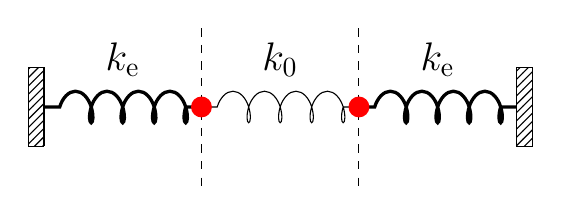
\begin{tikzpicture}
				\filldraw[pattern=north east lines] (0,-0.5) -| (-0.2,0.5) -| (0,-0.5);
				\filldraw[pattern=north east lines] (6,-0.5) -| (6.2,0.5) -| (6,-0.5);
				\draw[Spring] (0,0) -- (2,0);
				\draw[Spring, thin] (2,0) -- (4,0);
				\draw[Spring] (4,0) -- (6,0);
				
				\draw [dashed] (2,1) -- (2,-1);
				\draw [dashed] (4,1) -- (4,-1);
				
				\draw (2,0) node [fill=red,circle,scale=0.8] {};
				\draw (4,0) node [fill=red,circle,scale=0.8] {};
				
				\Large
				\draw (1,0.6) node [] {$k_\textrm{e}$};
				\draw (3,0.6) node [] {$k_0$};
				\draw (5,0.6) node [] {$k_\textrm{e}$};
			\end{tikzpicture}
			\label{fig: springs sym eq}}}

		\subfloat[Symmetric sloshing]{\scalebox{0.6}{
			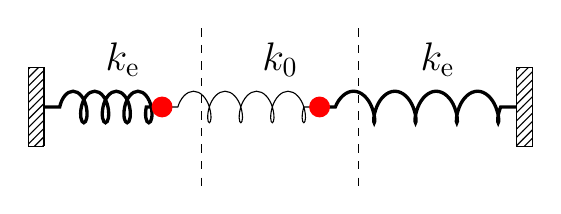
\begin{tikzpicture}
				\filldraw[pattern=north east lines] (0,-0.5) -| (-0.2,0.5) -| (0,-0.5);
				\filldraw[pattern=north east lines] (6,-0.5) -| (6.2,0.5) -| (6,-0.5);
				\draw[Spring] (0,0) -- (1.5,0);
				\draw[Spring, thin] (1.5,0) -- (3.5,0);
				\draw[Spring] (3.5,0) -- (6,0);
				
				\draw [dashed] (2,1) -- (2,-1);
				\draw [dashed] (4,1) -- (4,-1);
				
				\draw (1.5,0) node [fill=red,circle,scale=0.8] {};
				\draw (3.5,0) node [fill=red,circle,scale=0.8] {};
				
				\Large
				\draw (1,0.6) node [] {$k_\textrm{e}$};
				\draw (3,0.6) node [] {$k_0$};
				\draw (5,0.6) node [] {$k_\textrm{e}$};
			\end{tikzpicture}
			\label{fig: springs sym in-phase}}}

		\subfloat[Symmetric breathing]{\scalebox{0.6}{
			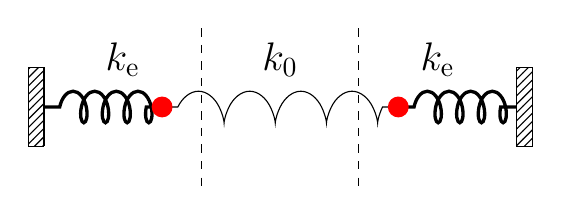
\begin{tikzpicture}
				\filldraw[pattern=north east lines] (0,-0.5) -| (-0.2,0.5) -| (0,-0.5);
				\filldraw[pattern=north east lines] (6,-0.5) -| (6.2,0.5) -| (6,-0.5);
				\draw[Spring] (0,0) -- (1.5,0);
				\draw[Spring, thin] (1.5,0) -- (4.5,0);
				\draw[Spring] (4.5,0) -- (6,0);
				
				\draw [dashed] (2,1) -- (2,-1);
				\draw [dashed] (4,1) -- (4,-1);
				
				\draw (1.5,0) node [fill=red,circle,scale=0.8] {};
				\draw (4.5,0) node [fill=red,circle,scale=0.8] {};
				
				\Large
				\draw (1,0.6) node [] {$k_\textrm{e}$};
				\draw (3,0.6) node [] {$k_0$};
				\draw (5,0.6) node [] {$k_\textrm{e}$};
			\end{tikzpicture}
			\label{fig: springs sym anti-phase}}}}
	\\
	\makebox[\textwidth][c]{
		\subfloat[Asymmetric equilibrium]{\scalebox{0.6}{
			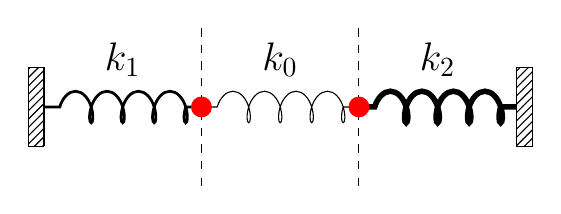
\begin{tikzpicture}
				\filldraw[pattern=north east lines] (0,-0.5) -| (-0.2,0.5) -| (0,-0.5);
				\filldraw[pattern=north east lines] (6,-0.5) -| (6.2,0.5) -| (6,-0.5);
				\draw[Spring, line width=1] (0,0) -- (2,0);
				\draw[Spring, thin] (2,0) -- (4,0);
				\draw[Spring, line width=2] (4,0) -- (6,0);
				
				\draw [dashed] (2,1) -- (2,-1);
				\draw [dashed] (4,1) -- (4,-1);
				
				\draw (2,0) node [fill=red,circle,scale=0.8] {};
				\draw (4,0) node [fill=red,circle,scale=0.8] {};
				
				\Large
				\draw (1,0.6) node [] {$k_1$};
				\draw (3,0.6) node [] {$k_0$};
				\draw (5,0.6) node [] {$k_2$};
			\end{tikzpicture}
			\label{fig: springs asym eq}}}

		\subfloat[Asymmetric sloshing]{\scalebox{0.6}{
			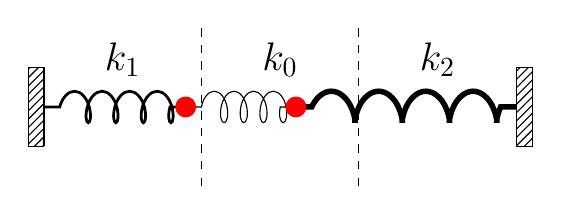
\begin{tikzpicture}
				\filldraw[pattern=north east lines] (0,-0.5) -| (-0.2,0.5) -| (0,-0.5);
				\filldraw[pattern=north east lines] (6,-0.5) -| (6.2,0.5) -| (6,-0.5);
				\draw[Spring, line width=1] (0,0) -- (1.8,0);
				\draw[Spring, thin] (1.8,0) -- (3.2,0);
				\draw[Spring, line width=2] (3.2,0) -- (6,0);
				
				\draw [dashed] (2,1) -- (2,-1);
				\draw [dashed] (4,1) -- (4,-1);
				
				\draw (1.8,0) node [fill=red,circle,scale=0.8] {};
				\draw (3.2,0) node [fill=red,circle,scale=0.8] {};
				
				\Large
				\draw (1,0.6) node [] {$k_1$};
				\draw (3,0.6) node [] {$k_0$};
				\draw (5,0.6) node [] {$k_2$};
			\end{tikzpicture}
			\label{fig: springs asym in-phase}}}

		\subfloat[Asymmetric breathing]{\scalebox{0.6}{
			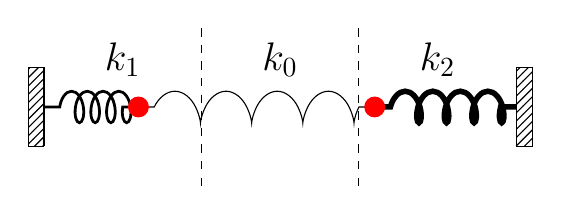
\begin{tikzpicture}
				\filldraw[pattern=north east lines] (0,-0.5) -| (-0.2,0.5) -| (0,-0.5);
				\filldraw[pattern=north east lines] (6,-0.5) -| (6.2,0.5) -| (6,-0.5);
				\draw[Spring, line width=1] (0,0) -- (1.2,0);
				\draw[Spring, thin] (1.2,0) -- (4.2,0);
				\draw[Spring, line width=2] (4.2,0) -- (6,0);
				
				\draw [dashed] (2,1) -- (2,-1);
				\draw [dashed] (4,1) -- (4,-1);
				
				\draw (1.2,0) node [fill=red,circle,scale=0.8] {};
				\draw (4.2,0) node [fill=red,circle,scale=0.8] {};
				
				\Large
				\draw (1,0.6) node [] {$k_1$};
				\draw (3,0.6) node [] {$k_0$};
				\draw (5,0.6) node [] {$k_2$};
			\end{tikzpicture}
			\label{fig: springs asym anti-phase}}}}

	\caption{A coupled mechanical oscillator gives an analogy to the eigenmodes of symmetric and asymmetric magnetic slabs. Spring constants are denoted $k$, with a thicker spring corresponding to a higher spring constant. Figures~(a) and~(d) show the symmetric and asymmetric spring systems in equilibrium. Figures~(b) and~(c) show the normal modes of a symmetric system. Figures~(e) and~(f) show the normal modes of an asymmetric system with spring constants $k_2 > k_1$. In each panel, the vertical dashed lines give the positions of the red masses at equilibrium.}
	\label{fig: springs all}
\end{figure}


%------------------------------------------------------------------------------
\section{Asymmetric slab in a magnetic environment}
\label{sec: EVP mag}
%------------------------------------------------------------------------------

Now we return to the general model for a magnetic slab, that is, a magnetic slab with asymmetric external environment.

\subsection{Summary of the eigenmode}

The eigenmodes and their dispersion is broadly similar to the slab in a non-magnetic environment. The differences, where they exist, are briefly discussed here.

\begin{figure}[]
	\centering
	\subfloat[$v_{A0} > c_0$]{\includegraphics[scale=0.45]{\figdir disp-mag-outside-photophere.png}
		\label{fig: disp mag 1}}
	\subfloat[$v_{A0} < c_0$]{\includegraphics[scale=0.45]{\figdir disp-mag-outside-2.png}
		\label{fig: disp mag 2}}
	\caption{Dispersion diagram for the dispersion relation, Equation~\eqref{DR}. \textcolor{red}{Finish}}
	\label{fig: disp mag}
\end{figure}


\subsection{Implications for observations}

Accurate mode identification is a key aspect of SMS. Different modes can differ in characteristics such as damping rate, phase and group speed, and, most relevant to this Thesis, response to waveguide asymmetry. Therefore, inaccurate mode identification can lead to significant error in diagnosis of background parameters. This subsection warns observational solar physicists of two possible ways in which errors in mode identification  could be made due to waveguide asymmetry.


\subsubsection{Quasi-symmetric eigenmodes}

It is possible for asymmetric MHD waves to have similar observational qualities to symmetric MHD waves. This can occur when the restoring force of perturbations (that is, the sum of the pressure gradient and Lorentz forces) is equal at both interfaces. This can occur in an asymmetric slab when the asymmetry in the pressure gradient force is precisely balanced to the asymmetry in the Lorentz force. We define these as \textit{quasi-symmetric} modes.

More precisely, we define quasi-symmetric modes to be eigenmodes which have equal transverse displacement amplitude on each boundary of the slab. This is equivalent to setting $\hat{v}_x (-x_0) = - \hat{v}_x (x_0)$ for quasi-sausage modes and $\hat{v}_x (-x_0) = \hat{v}_x (x_0)$ for quasi-kink modes.

The aim here is to prove that the necessary and sufficient condition for the existence of quasi-symmetric eigenmodes of an asymmetric magnetic slab is
\begin{equation}
\frac{\rho_1}{m_1}(k^2v_{A1}^2 - \omega^2) = \frac{\rho_2}{m_2}(k^2v_{A2}^2 - \omega^2), \label{quasi-sym condition}
\end{equation}
for a given frequency, $\omega$, and wavenumber, $k$.

To show that Equation~\eqref{quasi-sym condition} is sufficient for there to exist quasi-symmetric modes, consider an asymmetric magnetic slab with parameters that satisfy Equation~\eqref{quasi-sym condition}. Under this supposition, the transverse velocity perturbation solution for quasi-sausage modes reduces to
\begin{equation}
\hat{v}_x(x) =
\begin{cases}
A(\cosh{m_1x} + \sinh{m_1x}) & \text{if } x < -x_0, \\
C\sinh{m_0x} & \text{if } |x| \leq x_0, \\
D(\cosh{m_2x} - \sinh{m_2x}) & \text{if  } x > x_0,
\end{cases}
\end{equation}
where
\begin{equation}
A = \frac{-Cs_0}{c_1 - s_1}, \quad
D = \frac{Cs_0}{c_2 - s_2}, \quad
C \text{ is arbitrary}.
\end{equation}
The solution within the slab, $|x| \leq x_0$, is an odd function of $x$, therefore $\hat{v}_x(x_0) = -\hat{v}_x(-x_0)$. Therefore Equation~\eqref{quasi-sym condition} is a sufficient condition for the existence of quasi-symmetric modes. For quasi-kink modes, a similar proof is followed, where we find that $\hat{v}_x(x)$ is an even function within the slab.

To show that Equation~\eqref{quasi-sym condition} is necessary for there to exist quasi-symmetric modes, consider an asymmetric magnetic slab which supports quasi-symmetric modes. The transverse velocity perturbation solution is given by
\begin{equation}
\hat{v}_x(x) =
\begin{cases}
A(\cosh{m_1x} + \sinh{m_1x}) & \text{if } x < -x_0, \\
B\cosh{m_0x} + C\sinh{m_0x} & \text{if } |x| \leq x_0, \\
D(\cosh{m_2x} - \sinh{m_2x}) & \text{if } x > x_0, \label{vsoln}
\end{cases}
\end{equation}
where
\begin{align}
A &= \frac{1}{c_1 - s_1}(Bc_0 - Cs_0), \label{constA C} \\ 
D &= \frac{1}{c_2 - s_2}(Bc_0 + Cs_0), \label{constD C} \\
B &= \frac{\Lambda_0c_0 + \Lambda_1s_0}{\Lambda_0s_0 + \Lambda_1c_0}C = -\frac{\Lambda_0c_0 + \Lambda_2s_0}{\Lambda_0s_0 + \Lambda_2c_0}C, \label{constB C} \\
C & \text{ is arbitrary},
\end{align}
for quasi-sausage modes, and
\begin{align}
A &= \frac{1}{c_1 - s_1}(Bc_0 - Cs_0), \label{constA B} \\ 
D &= \frac{1}{c_2 - s_2}(Bc_0 + Cs_0), \label{constD B} \\
C &= \frac{\Lambda_0s_0 + \Lambda_1c_0}{\Lambda_0c_0 + \Lambda_1s_0}B = -\frac{\Lambda_0s_0 + \Lambda_2c_0}{\Lambda_0c_0 + \Lambda_2s_0}B, \label{constB B} \\
B & \text{ is arbitrary},
\end{align}
for quasi-kink modes. Given the supposition that the slab supports quasi-symmetric modes, we have, for quasi-sausage modes,
\begin{align}
\hat{v}_x(-x_0) &= -\hat{v}_x(x_0), \\
\implies \left(\frac{\Lambda_0c_0 + \Lambda_1s_0}{\Lambda_0s_0 + \Lambda_1c_0}\right) c_0 - s_0 &= -\left(\frac{\Lambda_0c_0 + \Lambda_1s_0}{\Lambda_0s_0 + \Lambda_1c_0}\right)c_0 - s_0, \\
\implies \Lambda_0c_0 + \Lambda_1s_0 &= 0.
\end{align}
Similarly, taking the second expression for $B$, we deduce that 
\begin{equation}
\Lambda_0c_0 + \Lambda_2s_0 = 0.
\end{equation}
It follows that $\Lambda_1 = \Lambda_2$, which is equivalent to Equation~\eqref{quasi-sym condition}, which concludes the proof that it is a necessary condition for the existence of quasi-symmetric quasi-sausage modes. For quasi-kink modes, a similar proof can be followed to show that $\hat{v}_x(x_0) = \hat{v}_x(-x_0)$ implies Equation~\eqref{quasi-sym condition}.






If we further specify that the penetration depth of perturbations in the external plasma be equal on each side of the slab, so that the eigenfunction is fully symmetric, then this implies that the external parameters are equal and we have a symmetric slab.

The main corollary to this result is that one can not conclude from an observation of a symmetric-looking MHD wave that the underlying waveguide is symmetric. This fallacy has been made in a number of previous studies (CITE) and could have lead to incorrect mode identification or diagnosis of the background plasma.

The question is then this: \textit{is it possible to differentiate between a symmetric and a quasi-symmetric eigenmode?} The answer to this is unclear. Theoretically, the answer is \textit{yes}. Although quasi-symmetric modes have symmetric amplitudes at the boundaries, they have asymmetric penetration depths into the external plasmas \textcolor{red}{(consider making a figure to show this in python)}. In theory, one could track the attenuation of the oscillation amplitude of plasma further away from the slab on each side. If the attenuation is asymmetric, the mode is quasi-symmetric. In practice, however, this will prove difficult. Although we currently have the required spatial resolution for measuring the spatial attenuation of MHD waves in many solar waveguides, the waveguides are unlikely to be isolated enough to allow for good measurements of this.


\subsubsection{Asymmetric mode or superposition of symmetric modes?}

A second implication that asymmetric eigenmodes have on mode identification in solar observations is that a waveguide oscillating in an asymmetric mode could be indistinguishable from a superposition of symmetric eigenmodes.

Consider how one has traditionally identified sausage and kink eigenmodes of a symmetric waveguide. To identify sausage modes, it has been presumed sufficient to identify oscillation in the cross-sectional width. To identify kink modes, it has been presumed sufficient to identify oscillation in the waveguide axis \textcolor{red}{(CITE?)}. The mixed characteristics of sausage and kink modes in asymmetric waveguides (see Table~\ref{tab: eigenmode differences}) tell us that these two characteristics are \textit{necessary} but not \textit{sufficient} for identification of the respective modes.

To appreciate the potential misidentification, consider a hypothetical observation of a waveguide in the solar atmosphere from which oscillations can be identified in both the cross-sectional width and the axis (for example, Figure~\ref{}, which uses the same dataset analysed by \cite{mor12}). If the oscillation is linear, the naive approach is to assume that the waveguide is symmetric, so that the only explanation for the cross-sectional oscillation is a symmetric sausage mode and the only explanation for the axial oscillation is a symmetric kink mode. One might then conclude that the observation is of a superposition of a sausage mode and a kink mode. However, 

One possible resolution to this problem is to measure the background parameters on each side of the waveguide to determine the degree of asymmetry before identifying the modes. If the waveguide is determined to be symmetric, symmetric modes can be identified. If not, the more general asymmetric modes can be identified.

One problem with this approach is that determining the key background parameters, the density and magnetic field strength, is often very difficult and estimates will have an associated uncertainty large enough that it would often not be possible to rule out the possibility of asymmetry. Another problem with this approach is that even relatively small degrees of waveguide asymmetry can cause significant asymmetry in the eigenmodes. For example, Figure~\ref{} gives a case where the ratio of the external densities is only \textcolor{red}{<CHANGE ME>}, yet the asymmetry in the eigenmodes (measured for example by the ratio of the oscillation amplitudes at each interface) is sufficient to show up in observations.

A second resolution is to independently measure the propagation speeds of the cross-sectional width oscillation and axial oscillation. Distinct eigenmodes propagate at distinct phase speeds\footnote{This is because of the uniqueness of eigenvalues in Sturm-Liouville systems \citep{boy_etal12}.}. If, in fact, the observation is of a superposition of symmetric sausage and kink eigenmodes, then each eigenmode will propagate at a distinct phase speed. Specifically, the cross-sectional oscillation will propagate at a different speed to the axial oscillation, and the oscillations will become out of phase. Whereas, if the oscillations in cross-sectional width and axis are both due to a single asymmetric eigenmode, then they will both share the same propagation speed and remain in phase. If different propagation speeds between these oscillation can be identified, then it will more likely be a superposition of symmetric modes than asymmetric modes.

One problem with this approach is that often only a small number of periods are observed before either the wave is damped or the waveguide disappears from observational view or breaks up. A notable exception to this are decayless kink oscillations \citep{nis_etal13}. When only a small number of periods are observed, there are often either too few periods to observe the cross-sectional width oscillations to become out of phase with axial oscillations, or errors in the phase-speed measurements too large to determine a difference. A second problem is that for some equilibrium parameters, the phase speeds of the symmetric sausage and kink eigenmodes are very similar. For example, this is true for body modes in most parameter regimes and for surface modes in a wide slab (Figure~\ref{} \textcolor{red}{Include a figure of symmetric slab dispersion diagrams}).



\appendix
\section{Coupled oscillator asymmetric eigenmodes} \label{app: coupled oscillator modes}
In this appendix, we prove that the breathing mode has highest amplitude on the mass connected to the external spring with lowest spring constant and the sloshing mode has highest amplitude on the mass connected to the external spring with highest spring constant.

Without loss of generality, let $\omega_2 > \omega_1$, so that the spring on the right has higher spring constant than the spring on the left. First, consider the case when $W < 1$. For the breathing mode, which has eigenfrequency $\omega_+$,
\begin{align}
	\left| \frac{\hat{x}_1}{\hat{x}_2} \right| & = \frac{1}{2W} \left(1 + \sqrt{1 + 4W^2}\right) \\
	& >  \frac{1}{2} \left(1 + \sqrt{1}\right), \quad \text{since $0 < W < 1$,} \\
	& = 1.
\end{align}
Therefore, the oscillation amplitude of the mass on the left is higher. For the sloshing mode, which has eigenfrequency $\omega_-$,
\begin{align}
	\left| \frac{\hat{x}_1}{\hat{x}_2} \right| & = \frac{1}{2W} \left|1 - \sqrt{1 + 4W^2}\right| \\
	& = \frac{1}{2W} \left(\sqrt{1 + 4W^2} - 1\right) \\
	& \leq \frac{1}{2W} \left(\sqrt{1} + \sqrt{4W^2} - 1\right), \quad \text{by the triangle inequality,} \\
	& = 1.
\end{align}
Therefore, the oscillation amplitude of the mass on the right is higher.

Next, consider the case when $W > 1$. For the breathing mode,
\begin{align}
\left| \frac{\hat{x}_1}{\hat{x}_2} \right| & = \frac{1}{2W} \left(1 + \sqrt{1 + 4W^2}\right) \\
& \geq \frac{1}{2W} \sqrt{2 + 4W^2}, \quad \text{by the triangle inequality,} \\
& = \sqrt{\frac{1}{2W} + 1} \\
& > 1,  \quad \text{since $W > 0$.}
\end{align}
Therefore, the oscillation amplitude of the mass on the left is higher. For the sloshing mode,
\begin{align}
\left| \frac{\hat{x}_1}{\hat{x}_2} \right| & = \frac{1}{2W} \left(\sqrt{1 + 4W^2} - 1\right) \\
& \leq \frac{1}{2W} \left(\sqrt{1 + 4W^2 - 1}\right), \quad \text{by the reverse triangle inequality,} \\
& = 1.
\end{align}
Therefore, the oscillation amplitude of the mass on the right is higher.

Finally, it is trivial to show the same result holds in the case where $W = 1$. This completes the proof that the breathing mode has highest amplitude on the mass connected to the external spring with lowest spring constant and the sloshing mode has highest amplitude on the mass connected to the external spring with highest spring constant.


\bibliographystyle{agsm}
\bibliography{../main/references}  

\end{document}
